\newif\iffull
\newif\ifnotfull
\fulltrue % Set \fulltrue to get the full version
\iffull
\notfullfalse
\else
\notfulltrue
\fi

\iffull % use article style for full version
\documentclass[11pt]{article}
%\usepackage[toc]{multitoc}
%\usepackage{times}
%\usepackage[affil-it]{authblk}
%\newcommand{\pubinfo}[1]{
%	\begin{figure}[!t] \vspace*{-5ex} #1\end{figure}}
\usepackage{fullpage}
%\usepackage[stable]{footmisc}
\usepackage{amsthm}
%\usepackage{mathptmx}
%\usepackage{lmodern}
%\usepackage{tikz}
\usepackage{float}
\usepackage{geometry}
\usepackage{protocolj}
%\usetikzlibrary{arrows,decorations.pathmorphing,decorations.footprints,
%	fadings,calc,trees,mindmap,shadows,decorations.text,patterns,positioning,
%	shapes,matrix,fit}
\newtheorem{theorem}{Theorem}
\newtheorem{lemma}{Lemma}
\newtheorem{claim}{Claim}
\theoremstyle{definition}
\newtheorem{definition}{Definition}
\newtheorem*{remark}{Remark}
\newenvironment{proofsk}{\begin{proof}[Proof (Sketch)]}{\end{proof}}

\else % use llncs format for short version
\documentclass[10pt,orivec]{llncs}
%\usepackage{fullpage}
\newenvironment{proofsk}{\begin{proof}[Proof (Sketch)]}{\end{proof}}
\newenvironment{prop}{\begin{proposition}}{\end{proposition}}
\usepackage{protocolj}
\fi

% packages
\usepackage{amsfonts,amssymb,amsmath,sectsty,url,float,enumitem}
%\usepackage[letterpaper,hmargin=.77in,vmargin=.77in]{geometry}

%\usepackage[pdfstartview=FitH,colorlinks,linkcolor=black,filecolor=black,citecolor=black,
%urlcolor=black]{hyperref}
%\usepackage{graphicx}
%%\usepackage{stackrel}
%\usepackage{ifpdf}
%\usepackage{multirow}
%\usepackage{relsize}
%\usepackage{multicol,color}
%\usepackage{amsbsy}
%\usepackage{ragged2e}
\usepackage{tikz}

\usepackage{amsfonts,amssymb,amsmath,sectsty,url,float,enumitem}
%\usepackage[letterpaper,hmargin=.77in,vmargin=.77in]{geometry}

%\usepackage[pdfstartview=FitH,colorlinks,linkcolor=black,filecolor=black,citecolor=black,
%urlcolor=black]{hyperref}
\usepackage{graphicx}
%\usepackage{stackrel}
\usepackage{ifpdf}
\usepackage{multirow}
\usepackage{relsize}
\usepackage{multicol,color}
\usepackage{amsbsy}
\usepackage{ragged2e}
%\usepackage[colorlinks = false]{hyperref}
\usepackage{hyperref}
\hypersetup{
    colorlinks=true, %set true if you want colored links
    linktoc=all,     %set to all if you want both sections and subsections linked
    linkcolor=red,  %choose some color if you want links to stand out
    citecolor=blue,
}

\urldef{\mailsc}\path|{antigoni}@cs.au.dk|  

\newtheorem{thm}{Theorem}
%\newcommand{\BT}{\begin{thm}}   \newcommand{\ET}{\end{thm}}
%\newtheorem{dfn}[thm]{Definition}      %
%\newcommand{\BD}{\begin{dfn}}   \newcommand{\ED}{\end{dfn}}
%\newtheorem{corr}[thm]{Corollary}      %
%\newcommand{\BCR}{\begin{corr}} \newcommand{\ECR}{\end{corr}}
%---
\newcommand{\BT}{\begin{thm}}   \newcommand{\ET}{\end{thm}}
\newtheorem{dfn}{Definition}      %
\newcommand{\BD}{\begin{dfn}}   \newcommand{\ED}{\end{dfn}}
\newtheorem{corr}{Corollary}      %
\newcommand{\BCR}{\begin{corr}} \newcommand{\ECR}{\end{corr}}
%%%%%%
\newtheorem{Ithm}{Theorem}[section]     % A counter for Theorems in Intro
\newcommand{\BIT}{\begin{Ithm}}   \newcommand{\EIT}{\end{Ithm}}
%---
\newtheorem{lem}{Lemma}[section]  % A counter for Lemmas etc
\newcommand{\BL}{\begin{lem}}   \newcommand{\EL}{\end{lem}}
%\newtheorem{prop}[lem]{Proposition}
\newcommand{\BP}{\begin{prop}}   \newcommand{\EP}{\end{prop}}
\newtheorem{clm}{Claim}            %
\newcommand{\BCM}{\begin{clm}}   \newcommand{\ECM}{\end{clm}}
\newtheorem{fact}[lem]{Fact}            %
\newcommand{\BF}{\begin{fact}}   \newcommand{\EF}{\end{fact}}
\renewenvironment{proof}{\noindent{\bf Proof:~~}}{\qed}
\newcommand{\BPF}{\begin{proof}} \newcommand {\EPF}{\end{proof}}

\newcommand{\BPR}{\begin{prot}}   \newcommand{\EPR}{\end{prot}}
\newenvironment{cproof}{\noindent{\bf Proof:~~}}{\hfill $\Box$}
\newcommand{\BCPF}{\begin{cproof}} \newcommand {\ECPF}{\end{cproof}}
\newcommand{\Qed}{\hfill $\Box$}

%\newtheorem{remark}[lem]{Remark}
\newcommand{\BR}{\begin{remark}}   \newcommand{\ER}{\end{remark}}

\newcommand{\BDE}{\begin{description}}
\newcommand{\EDE}{\end{description}}
\newcommand{\BE}{\begin{enumerate}}
\newcommand{\EE}{\end{enumerate}}
\newcommand{\BI}{\begin{itemize}}
\newcommand{\EI}{\end{itemize}}
\newcommand{\BEQ}{\begin{eqnarray*}}
\newcommand{\EEQ}{\end{eqnarray*}}
\newcommand{\nmcom}{\nmCom}
%\newcommand{\sectionbreak}{}

%%%%%%%%%%%%%%%%%%%%%%%%%%%%%%%%%%%%%%%%%%%%%%%%%%%%%%%%%%%%%%%%%%%%%%
%%%%%%%%%%%%%%%%%%%%   DOCUMENT BEGINS HERE   %%%%%%%%%%%%%%%%%%%%%%%%
%%%%%%%%%%%%%%%%%%%%%%%%%%%%%%%%%%%%%%%%%%%%%%%%%%%%%%%%%%%%%%%%%%%%%%

\title{Four Round Secure Computation without Setup}
%\title{Secure Computation in Four Rounds Without Trusted Setup via Multi-Key FHE}
\date{}
\iffull
\author{Zvika Brakerski\thanks{Supported by the Israel Science Foundation (Grant No.\ 468/14), Alon Young Faculty Fellowship and Binational Science Foundation (Grant No.\ 712307).}  \\ Weizmann Institute of Science
\and Shai Halevi\thanks{Supported by the Defense Advanced Research Projects Agency (DARPA) and Army Research Office(ARO) under Contract No. W911NF-15-C-0236.} \\ IBM
\and Antigoni Polychroniadou\thanks{Supported by the National Science Foundation under Grant No. 1617676, IBM under Agreement 4915013672, the Packard Foundation under Grant 2015-63124, and the Danish National Research Foundation and the National Science Foundation of China (under the grant 61361136003) for the Sino-Danish Center for the Theory of Interactive Computation. Any opinions, findings, and conclusions or recommendations expressed in this material are those of the author(s) and do not necessarily reflect the views of the sponsors.}  \\ Cornell Tech
}

\else
\author{}
\fi

% !TEX root =./main-optimal.tex
%\newcommand{\figref}[1]{Figure~\ref{fig:#1}}
\newcommand{\figlab}[1]{\label{fig:#1}}
\def\calA{\mathcal{A}}
\def\calB{\mathcal{B}}
\def\calC{\mathcal{C}}
\def\calD{\mathcal{D}}

\newcommand{\thmref}[1]{Theorem~\ref{thm:#1}}
\newcommand{\corref}[1]{Corollary~\ref{cor:#1}}
\newcommand{\lemref}[1]{Lemma~\ref{lem:#1}}
\newcommand{\tblref}[1]{Table~\ref{tbl:#1}}
\newcommand{\figref}[1]{Figure~\ref{fig:#1}}
\newcommand{\secref}[1]{Section~\ref{sec:#1}}
\newcommand{\appref}[1]{Appendix~\ref{app:#1}}
\newcommand{\eqnref}[1]{Eqn.~(\ref{eqn:#1})}
\newcommand{\defref}[1]{Definition~\ref{def:#1}}

\newcommand{\func}{\mathcal{F}}
\newcommand{\nmc}{\mathsf{nmc}}
\newcommand{\tagg}{\mathsf{tag}}
\newcommand{\rnm}{\ensuremath{k}}
\newcommand{\id}{\ensuremath{\mathsf{id}}}
\newcommand{\oid}{\ensuremath{{\mathsf{{tag}}}}}
\newcommand{\pok}{\ensuremath{\mathsf{pok}}}
\newcommand{\st}{\ensuremath{\mathsf{st}}}
\newcommand{\theo}{\ensuremath{\mathsf{th}}}
\newcommand{\thmm}{\ensuremath{\mathsf{thm}}}
\newcommand{\prg}{\ensuremath{\mathsf{prg}}}
\newcommand{\tthm}{\ensuremath{\mathsf{{\widetilde{thm}}}}}
\newcommand{\dist}{{\cal D}}	
\newcommand{\compind}{\approx_{\mathrm{c}}}
\newcommand{\statind}{\approx_{\mathrm{s}}}
\newcommand{\ok}{\ensuremath{\mathsf{eqthm}}}
\newcommand{\otm}{\mathsf{OTMsg}}
\newcommand{\wipokm}{\mathsf{WIPoKMsg}}
\newcommand{\idind}{\equiv}
\newcommand{\zkakm}{\mathsf{ZKAKMsg}}
\newcommand{\Lab}{\mathsf{L}}
\newcommand{\gc}{\mathsf{GC}}
\newcommand{\tld}{\widetilde}
\newcommand{\Ideal}{\textsc{IDEAL}}
\newcommand{\LWE}{\textsc{LWE}}
%%%%%%%%%%%%%%%%%%%%%%%%%%
% Calligraphical Alphabet %
%%%%%%%%%%%%%%%%%%%%%%%%%%
\newcommand{\cA}{{\cal A}}
\newcommand{\cVa}{{\mathcal I_\Com}}
\newcommand{\cIVa}{{\mathcal J_\Com}}
\newcommand{\cB}{{\cal B}}
\newcommand{\cC}{{\cal C}}
\newcommand{\ccP}{{\cal P}}
\renewcommand{\P}{{P}}

\newcommand{\SSS}{{\cal SS}}

\newcommand{\cD}{{\cal D}}
\newcommand{\cE}{{\cal E}}
\newcommand{\cF}{{\cal F}}
\newcommand{\cG}{{\cal G}}
\newcommand{\cH}{{\cal H}}
\newcommand{\cI}{{\cal I}}
\newcommand{\cK}{{\cal K}}
\newcommand{\cL}{{\cal L}}
\newcommand{\cM}{{\cal M}}
\newcommand{\cN}{{\cal N}}
\newcommand{\cO}{{\cal O}}

\newcommand{\cQ}{{\cal Q}}
\newcommand{\cR}{{\cal R}}
\newcommand{\cS}{{\cal S}}
\newcommand{\NP}{{{\cal NP}}}
\newcommand{\cT}{{\cal T}}
\newcommand{\cU}{{\cal U}}
\newcommand{\cV}{{\cal V}}
\newcommand{\cX}{{\cal X}}
\newcommand{\cY}{{\cal Y}}
\newcommand{\cZ}{{\cal Z}}
\newcommand{\cW}{{\cal W}}

%%%%%%%%%%%%%%%%%%%%%%%%%%%%
% Blackboard Bold Alphabet %
%%%%%%%%%%%%%%%%%%%%%%%%%%%%
\renewcommand{\AA}{\mathbf{A}}
\newcommand{\CC}{\mathbb{C}}
\newcommand{\E}{\mathbb{E}}
\newcommand{\FF}{\mathbb{F}}
\newcommand{\GG}{\mathbb{G}}
\newcommand{\HH}{\mathbb{H}}
\newcommand{\NN}{\mathbb{N}}
\newcommand{\PP}{\mathbb{P}}
\newcommand{\QQ}{\mathbb{Q}}
\newcommand{\RR}{\mathbb{R}}
\newcommand{\ZZ}{\mathbb{Z}}

%%%%%%%%%%%%%%%%%%%%%%%%%%
% Boldface Math Alphabet %
%%%%%%%%%%%%%%%%%%%%%%%%%%
\def \bfa{{\mathbf a}}
\def \bfb{{\mathbf b}}
\def \bfc{{\mathbf c}}
\def \bfe{{\mathbf e}}
\def \bff{{\mathbf f}}
\def \bfg{{\mathbf g}}
\def \bfm{{\mathbf m}}
\def \bfp{{\mathbf p}}
\def \bfr{{\mathbf r}}
\def \bfs{{\mathbf s}}
\def \bft{{\mathbf t}}
\def \bfu{{\mathbf u}}
\def \bfv{{\mathbf v}}
\def \bfw{{\mathbf w}}
\def \bfx{{\mathbf x}}
\def \bfy{{\mathbf y}}
\def \bfz{{\mathbf z}}
\def \bfA{{\mathbf A}}
\def \bfH{{\mathbf H}}
\def \bfZ{{\mathbf Z}}
\def \bfS{{\mathbf S}}



\newcommand{\sprot}{\prot^\simul}
\newcommand{\spar}{\kappa}
\newcommand{\prot}{\mathrm{\Pi}}
\newcommand{\cfprot}{\prot_{\sf flip}}
\newcommand{\cfprots}{\prot_{\sf flip}^{\simul}}
\newcommand{\cfprotn}{\prot_{\sf flip}^{\nosimul}}
\newcommand{\simul}{\Leftrightarrow}
\newcommand{\nosimul}{{\stackrel{\leftarrow}{\rightarrow}}}
\newcommand{\pno}{n}
\newcommand{\advS}{\cS}
\newcommand{\rlen}{\lambda}
\newcommand{\tc}{\widetilde{c}}
\newcommand{\msg}{\mathsf{m}}
\newcommand{\mprot}[4]{\msg_{#1,#2}^{#3[#4]}}
\newcommand{\rd}{\mathsf{\rho}}
%\newcommand{\Sim}{\advS}
\newcommand{\tP}{{\P}^\simul}
\newcommand{\tSimu}{\advS^{\simul}}
\newcommand{\cor}[1]{\overline{#1}}
\newcommand{\cP}{\cor{\P}}

\newcommand{\Simu}{\cS}
\newcommand{\view}{\mathsf{view}}
\newcommand{\real}{\textsc{REAL}}
\newcommand{\extended}{\text{Extended}}


% New commands


\def \GCircuit {\ensuremath\mathsf{GenGC}}
\def \Eval {\ensuremath\mathsf{EvalGC}}

\def \lab {\ensuremath{lab}}
\def \lbl {\ensuremath{Z}}
\def \tlbl {{\widetilde{\ensuremath{Z}}}}
\def \sec {\kappa}
\def \inp {\ensuremath\mathsf{wires}}
\newcommand{\inpsz}{n}
\def \CircSim {\ensuremath\mathsf{SimGC}}
\def \out {\ensuremath\mathsf{out}}

	\newcommand{\sig}{\textsf{Sig}}
\newcommand{\tid}{\textsf{mid}}
\newcommand{\create}{\textsf{create}}
\newcommand{\run}{\textsf{run}}



\newcommand{\piOT}{\ensuremath{\mathrm{\Pi_\ot}}}

\newcommand{\Com}{\ensuremath{\mathsf{bCom}}}
\newcommand{\qCom}{\ensuremath{\mathsf{Eqcom}}}
\newcommand{\eCom}{\ensuremath{\mathsf{Extcom}}}
\newcommand{\nmCom}{\ensuremath{\mathsf{aCom}}}
\newcommand{\open}{\ensuremath{\mathsf{open}}}
\newcommand{\topen}{{\widetilde{\mathsf{open}}}}
\newcommand{\tsigma}{{\widetilde{\mathsf{\sigma}}}}
\newcommand{\tCom}{\ensuremath{\widehat{\mathsf{com}}}}

\newcommand{\hb}{\mathsf{H}}
\newcommand{\Ext}{\mathsf{Ext}}
\newcommand{\sCom}{\mathsf{SCom}}
\newcommand{\com}{\mathsf{com}}
\newcommand{\scom}{\mathsf{scom}}
\newcommand{\decom}{\mathsf{decom}}
\newcommand{\tcom}{\mathsf{tcom}}
\newcommand{\Open}{\mathsf{Open}}
\newcommand{\TCom}{\mathsf{TCom}}
\newcommand{\TCmsg}{\mathsf{TCmsg}}
\newcommand{\OTmsg}{\mathsf{OTmsg}}
\newcommand{\WIPOKmsg}{\mathsf{p}}
\newcommand{\FLSmsg}{\mathsf{fs}}
\newcommand{\tWIPOKmsg}{{\widetilde{\mathsf{p}}}}
\newcommand{\tFLSmsg}{{\widetilde{\mathsf{fs}}}}

\newcommand{\TCdecom}{\mathsf{TCdecom}}
\newcommand{\TOpen}{\mathsf{TOpen}}
\newcommand{\Share}{\mathsf{Share}}
\newcommand{\Rec}{\mathsf{Recon}}
\newcommand{\valid}{\mathsf{valid}}
\newcommand{\noi}{\noindent}
\newcommand{\vw}{{\bf D}}

\newcommand{\remove}[1]{}
\newcommand{\Setup}{{\mathsf{MFHE.Setup}}}
\newcommand{\DSetup}{{\mathsf{MFHE.DistSetup}}}
\newcommand{\pp}{{\mathsf{pp}}}
\newcommand{\gencom}{{\mathsf{GenCom}}}
\newcommand{\decommit}{{\mathsf{Decommit}}}
\newcommand{\Inv}{\mathsf{Inv}}
\newcommand{\PRF}{{\mathsf{PRF}}}
\newcommand{\Maj}{{\mathsf{Majority}}}
\newcommand{\TK}{{\mathsf{TK}}}
\newcommand{\Ver}{{\mathsf{Ver}}}

\newcommand{\WI}{\ensuremath{\mathsf{WI}}}
\newcommand{\nm}{\ensuremath{\mathsf{acom}}}
%\newcommand{\onm}{\ensuremath{\overline{\mathsf{nm}}}}
\newcommand{\onm}{\ensuremath{{\mathsf{bcom}}}}
\newcommand{\ecom}[1]{\ensuremath{\mathsf{C^{ex}_{#1}}}}
\newcommand{\tecom}[1]{\ensuremath\widetilde{{\mathsf{C^{ex}_{#1}}}}}
\newcommand{\lcom}{\mathsf{C}_{\mathsf{lab}}}
\newcommand{\gccom}{\mathsf{C}_{\mathsf{gc}}}
\newcommand{\tlcom}{\widetilde{\mathsf{C}}_{\mathsf{lab}}}
\newcommand{\tgccom}{\widetilde{\mathsf{C}}_{\mathsf{gc}}}
%\newcommand{\tgccom}{{{\widetilde{{\mathsf{C}}}_{{\mathsf gc}}}}}



\newcommand{\tnm}{{\widetilde{\mathsf{nm}}}}
\newcommand{\tr}{{\widetilde{{r}}}}
\newcommand{\tz}{{\widetilde{{z}}}}
\newcommand{\tw}{{\widetilde{{\omega}}}}


\newcommand{\MFHE}{{\mathsf{MFHE}}}
\newcommand{\CPA}{{\mathsf{CPA}}}



%\newcommand{\onest}{{\cL_1^{i,j}}}
%\newcommand{\twost}{{\cL_2^{i,j}}}
%\newcommand{\threest}{{\cL_3^{i,j}}}
%\newcommand{\fourst}{{\cL_4^{i,j}}}

\newcommand{\onest}{{\cL_{i,j,1}}}
\newcommand{\twost}{{\cL_{i,j,2}}}
\newcommand{\threest}{{\cL_{i,j,3}}}
\newcommand{\fourst}{{\cL_{i,j,1}}}

\newcommand{\hhonest}{{\cL_{h,j,1}}}
\newcommand{\hhtwost}{{\cL_{h,j,2}}}
\newcommand{\hhstPOK}{{\cL^\WIPOK_{P_h}}}

\newcommand{\stFLS}{{{{\mathsf{\cL}}^{\FLS}_{P_i}}}}
\newcommand{\stFLSS}{{{{\mathsf{\cL}}^{\FLS}_{P_j}}}}
\newcommand{\sstFLS}{{{{\mathsf{\cL}}^{\FLS}_{P}}}}
\newcommand{\stPOK}{{\cL^\WIPOK_{P_i}}}
\newcommand{\sstPOK}{{\cL^\WIPOK_{P}}}


\newcommand{\honest}{{\cL_1^{h,j}}}
\newcommand{\htwost}{{\cL_2^{h,j}}}
\newcommand{\hthreest}{{\cL_3^{h,j}}}
\newcommand{\hstPOK}{{\cL_\WIPOK^{h,j}}}

\newcommand{\tonest}{{\widetilde{\mathsf{\cL_1}}}}
\newcommand{\ttwost}{{\widetilde{\mathsf{\cL_2}}}}
\newcommand{\tthreest}{{\widetilde{\mathsf{\cL_3}}}}
\newcommand{\tfourst}{{\widetilde{\mathsf{\cL_4}}}}
\newcommand{\tstFLS}{{\widetilde{\mathsf{\cL_\FLS}}}}
\newcommand{\tstPOK}{{\widetilde{\mathsf{\cL_\WIPOK}}}}


\newcommand{\zk}{{\mathsf{ZK}}}
\newcommand{\CF}{{\mathsf{CF}}}
\newcommand{\tV}{{\tilde{V}}}
\newcommand{\tE}{{\tilde{E}}}
%\newcommand{\tw}{{\tilde{w}}}
\newcommand{\tomega}{{\widetilde{\omega}}}
\newcommand{\ty}{{\tilde{y}}}
\newcommand{\tS}{{\tilde{S}}}
\newcommand{\tnu}{{\tilde{\nu}}}
\newcommand{\tC}{{\mathsf{GC}}}

\newcommand{\tl}{{\tilde{l}}}
\newcommand{\td}{{\tilde{d}}}
\newcommand{\tPi}{{\tilde{\Pi}}}
\newcommand{\ngl}{{\mathsf{negl}}}
\newcommand{\trans}{{\mathsf{trans}}}

\newcommand{\ideall}{\mbox{\textsc IDEAL}}
\newcommand{\hyb}{{\bf H}}
\newcommand{\thyb}{{\widetilde{\bf Hybrid}}}
\newcommand{\whyb}{{\overline{\bf Hybrid}}}

\newcommand{\hybs}{{\bf Hybrids}}
\newcommand{\reall}{\mbox{\textsc REAL}}
\newcommand{\eqdef}{\stackrel{\rm def}{=}}
\newcommand{\indist}{\stackrel{\rm c}{\approx}}
\newcommand{\deff}{\stackrel{\rm def}{=}}
\newcommand{\statclose}{\stackrel{\rm s}{\approx}}
\newcommand{\rnd}{\gets_R}
\newcommand{\ppt}{{\sc PPT}}
\newcommand{\prob}{{\rm Pr}}
\newcommand{\rec}{{P_j}}
\newcommand{\sen}{{P_i}}
\newcommand{\recc}{{A_2}}
\newcommand{\senn}{{A_1}}
\newcommand{\adv}{\textsc{Adv}}
\newcommand{\comp}{\textrm{Comp}}
\newcommand{\GPi}{\Pi^{\glb}}
\newcommand{\prf}{\mathrm{f}}
\newcommand{\rlcom}[1]{\mathsf{C^{{\sf eq}}_{#1}}}
\newcommand{\ct}{{\scriptscriptstyle\mathrm{CT}}}
\newcommand{\ot}{{\scriptscriptstyle\mathrm{OT}}}
\newcommand{\FLS}{{\scriptscriptstyle\mathrm{FS}}}
\newcommand{\WIPOK}{{\scriptscriptstyle\mathrm{WIPOK}}}


\newcommand{\PC}{{\scriptscriptstyle\mathrm{MPC}}}
\newcommand{\CFF}{{\scriptscriptstyle\mathrm{2CF}}}
\newcommand{\comm}{{\scriptscriptstyle\mathrm{COM}}}

\newcommand{\gate}{{\mathsf{Gate}}}
\newcommand{\enc}{\mathsf{Enc}}
\newcommand{\dec}{\mathsf{Dec}}
\newcommand{\gen}{\mathsf{Gen}}
\newcommand{\Gen}{{\mathrm{Gen}}}
\newcommand{\Evall}{{\mathsf{MFHE.Eval}}}
\newcommand{\Invert}{{\mathrm{Invert}}}



\newcommand{\Encrypt}{{\mathsf{MFHE.Encrypt}}}

\newcommand{\PartDec}{{\mathsf{MFHE.PartDec}}}
\newcommand{\FinDec}{{\mathsf{MFHE.FinDec}}}



\newcommand{\Decrypt}{\mathsf{MFHE.Decrypt}}
\newcommand{\Expand}{\mathsf{Expand}}
\newcommand{\Keygen}{\mathsf{MFHE.Keygen}}
%\newcommand{\Setup}{\mathsf{Setup}}
\newcommand{\params}{{\mathsf{params}}}
\newcommand{\pk}{{\mathsf{pk}}}
\newcommand{\PK}{{{B}}}
\newcommand{\sk}{{\mathsf{sk}}}
\newcommand{\hc}{{{\hat{c}}}}

\def\setupOne{{\sf Gen_1}}
\def\setupTwo{{\sf Gen_2}}


\newcommand{\ideal}{{\scriptscriptstyle\mathrm{IDEAL}}}
\newcommand{\hybrid}{{\scriptscriptstyle\mathrm{HYBRID}}}
\newcommand{\sh}{{\scriptscriptstyle\mathrm{SH}}}
\newcommand{\ml}{{\scriptscriptstyle\mathrm{ML}}}
\newcommand{\mext}{{\scriptscriptstyle\mathrm{mEXTCOM}}}
\newcommand{\ext}{{\scriptscriptstyle\mathrm{EXTCOM}}}


\newcommand{\code}{{\scriptscriptstyle\mathrm{code}}}
\newcommand{\bb}{{\scriptscriptstyle\mathrm{bb}}}
\newcommand{\set}{{\scriptscriptstyle\mathrm{TP}}}

\newcommand{\ucset}{{\scriptscriptstyle\mathrm{UCTP}}}
\newcommand{\uc}{{\scriptscriptstyle\mathrm{UC}}}
\newcommand{\Hyb}[1]{\mathrm{\mathrm{H}_{#1}}}
\newcommand{\tHyb}[1]{{\widetilde{\mathrm{\mathrm{H}}}_{#1}}}
\newcommand{\wHyb}[1]{{\overline{\mathrm{\mathrm{H}}}_{#1}}}












%\theoremstyle{plain}
%\newtheorem{innercustomlem}{Lemma}
%%
%\newenvironment{customlem}[1]
%{\renewcommand\theinnercustomlem{#1}\innercustomlem}
%{\endinnercustomlem}
%\newtheorem{innercustomthm}{Theorem}
%%
%\newenvironment{customthm}[1]
%{\renewcommand\theinnercustomthm{#1}\innercustomthm}
%{\endinnercustomthm}

%\newcommand{\set}[2]{\{#1,\ldots,#2\}}


\newcommand{\fail}{\texttt{fail}}



\newcommand{\advA}{\cA}

\newenvironment{boxfig}[2]{% {#1}{#2} = {Caption}{label}
     \begin{figure}[ht!]
     \newcommand{\FigCaption}{#1}
     \newcommand{\FigLabel}{#2}
       \vspace{-0.8cm}
     \begin{center}
       \begin{small}
         \begin{tabular}{@{}|@{~~}l@{~~}|@{}}
           \hline
           \rule[-1.5ex]{0pt}{1ex}\begin{minipage}[b]{1.09\linewidth}
             \vspace{1ex}
             \smallskip
             }{%
           \end{minipage}\\
           \hline
         \end{tabular}
       \end{small}
       \vspace{-0.4cm}
      \caption{\FigCaption}
       \figlab{\FigLabel}
     \end{center}
     \vspace{-0.4cm}
   \end{figure}
}


\renewcommand{\vec}[1]{\mathbf{#1}}
		
	
		\newcommand{\bit}{\{0,1\}}
		\newcommand{\twoPC}{\ensuremath{\mathsf{2PC}}}
			\newcommand{\MCF}{\ensuremath{\mathsf{MCF}}}
		

		
		\newcommand{\Comment}[2][red]{\marginpar{
				\fcolorbox{#1}{white}{\parbox{.8in}{
						\color{#1} \small \sf  #2 }}}}
		\newcommand{\mcomment}[2]{\textcolor{red}{#1}\Comment{#2}}
		\newcommand{\TODO}[2][\relax]{\noindent\mcomment{#2}{#1 TODO}}
		\newcommand{\mytodo}[2]{\mcomment{ #1 }{#2 TODO}}
	%\newcommand{\ucomment}[3]{\par\noindent{\textcolor{#1}{/* #2 */}}\Comment[#1]{// #3}}
	\newcommand{\ucomment}[3]{}
		
		\newcommand{\anti}[1]{\ucomment{blue}{#1}{Antigoni}}
		\newcommand{\shai}[1]{\ucomment{red}{#1}{Shai}}
		\newcommand{\anote}[1]{\ucomment{green}{#1}{Note:}}
				\newcommand{\znote}[1]{\ucomment{purple}{#1}{Z}}
		
		\pagestyle{plain}
		\sloppy
		\pagenumbering{arabic}




\begin{document}
\sloppy % Prevents stuff from hanging into margins
\maketitle

\begin{abstract}

\end{abstract}


\iffull
\else
\bigskip\paragraph{Keywords:} LWE, Multikey FHE, MPC, Round efficiency.
\fi

\iffull
\pagestyle{empty}
\newpage
\setcounter{tocdepth}{3}
\tableofcontents
\newpage
\setcounter{page}{1}
\pagestyle{plain}
\fi

%%%%%%%%%%%%%%%%%%%%%%%%%%%%%%%%%%%%%%%%%%%%%%%%%%%%%%%%%%%%%%%%%%%%%%
% !TEX root =../main-optimal.tex
\section{Introduction}
%%%%%%%%%%%%%%%%%%%%%%%%%%%%%%%%%%%%%%%%%%%%%%%%%%%%%%%%%%%%%%%%%%%%%%
Secure Multi-party Computation (MPC) \cite{FOCS:Yao82b,FOCS:Yao86,GMW87} allows mutually suspicious parties to evaluate a function on their joint private inputs without revealing these inputs to each other.
%\shai{a few paragraphs about round complexity, major prior works, current status. with/without setup, 2-party/multi-party, ordered/simultaneous, etc. In particular mention Mukherjee-Wichs \cite{MW16}.}
One particularly fruitful line of investigation is concerned with the \emph{round complexity} of these protocols, more specifically how many rounds of broadcast are needed.

There are many variants of this question, depending on the exact model. In particular, the availability (or lack thereof) of a \emph{Common Reference String} (CRS) plays an important role in the study of round complexity. It is known that at least two rounds of interaction are necessary even if such trusted CRS is available (e.g., \cite{C:HalLinPin11}), and several works in the literature construct optimal (two) round secure computation protocols both in the two-party and multi-party settings (see \secref{relatedCRS} for related works).

In the plain model without trusted setup, Katz and Ostrovsky \cite{C:KatOst04} proved that five rounds are necessary and sufficient for secure computation in the two-party setting where both parties rceive output. In the multi-party setting, it is long known that \emph{constant round protocols} are possible \cite{STOC:BeaMicRog90,EC:KatOstSmi03,STOC:Pass04,C:DamIsh05,C:DamIsh06,C:IshPraSah08,C:PanPasVai08,FOCS:Wee10,STOC:Goyal11,STOC:LinPas11,FOCS:GLOV12}, however there is no known round optimal multi-party computation protocol. 

In a recent work by Garg et al. \cite{EC:GMPP16}, it is shown that when simultaneous messages are allowed, then the Katz-Ostrovsky lower bound drops to only \emph{four} rounds (for either two or many parties). In terms of constructions, \cite{EC:GMPP16} show how to transform any $t$-round (parallel) non-malleable commitment into a $\max(4,t+1)$-round protocol for the specific coin-flipping functionality in the multi-party setting. Instantiating this protocol with the non-malleable commitments from \cite{C:PanPasVai08,C:COSV16}, Garg et al. obtained a four round protocol for the multi-party {\em coin-flipping} functionality. Relying on this coin-flipping protocol they showed how to transform the two-round multi-party protocol for general functionalities of Garg et al. \cite{TCC:GGHR14} based on indistinguishability Obfuscation (iO) \cite{FOCS:GGHRSW13} in the CRS model to a five-round protocol in the plain model, and the two-round LWE-based protocol of Mukherjee and Wichs \cite{MW16} to a six-round protocol.

A lot of work has been done on the round complexity of non-malleable commitments as well. However, the only candidates for parallel non-malleable commitments that run in less than four rounds are constructed in the works of \cite{C:PanPasVai08,C:COSV16}. The two round parallel non-malleable commitment of \cite{C:PanPasVai08} is based on adaptive pseudorandom generators (PRGs) and the three round non-malleable commitment of \cite{C:COSV16} is based on one-way permutations with sub-exponential security.

%Combining their coin flipping protocol with the $3$-round parallel non-malleable commitment of \cite {} or the 2-round parallel non-malleable commitment of \cite{C:PanPasVai08} they obtain a $4$ coin-flipping protocol. 

Even under very strong assumptions, prior works leave the following fundamental question open:
\begin{quote}
\emph{Can we obtain round-optimal multi-party computation protocols in the plain model (without setup)?}
\end{quote}

We answer the above question in the affirmative, obtaining a round-optimal multi-party computation protocol in the plain model for general functionalities in the presence of a malicious adversary. 
Our starting point is the observation that we can replace the four-round coin-tossing from \cite{EC:GMPP16} by an extremely simple \emph{single round protocol}. That protocol yeilds a common somewhat-random string, which is much weaker than a truly random string but still ``good enough for LWE''. This lets us run (a variant of) the Mukherjee-Wichs protocol \cite{MW16}, yeilding a three-round protocol with ``semi-malicious'' security, under the LWE assumption.

To get security in the malicious adversary model, we rely on other strong assumptions. In particular, we use the two-round adaptively secure commitment scheme of Pandey, Pass and Vaikuntanathan \cite{C:PanPasVai08} (which is just Naor's protocol from \cite{JC:Naor91}, when instantiated with adaptive PRGs). Moreover, we need a sub-exponential version of the LWE assumption. Hence, we prove the following:
\BT\label{thm:mpctoken}(Informal)
Assuming the existence of adaptive commitments, as well as the sub-exponential hardness of Learning-with-Errors, there exists a four-round protocol that securely realizes any multi-party functionality against a malicious adversary in the plain model without setup.
\ET

%Their non-malleable commitment is also the only $3$-robust parallel candidate that can be used in the $6$-round protocol of Garg et al. \cite{EC:GMPP16} from $\LWE$ together with the non-malleable commitment scheme of \cite{COSV16} which is based on complexity leveraging. 
\subsection {Related Work} \label{sec:relatedCRS}
\paragraph{Related work in the CRS model.}
The works of Jarecki and Shmatikov \cite{EC:JarShm07} and Horvitz and Katz~\cite{C:HorKat07} present {\em two-party} protocols where the former is constant-round and the latter is optimal (two)-round. Asharov et al.~\cite{EC:AJLTVW12} first show a three-round \emph{multi-party} computation protocol in the CRS model and a two-round multi-party computation protocol in the reusable PKI model, under LWE, by constructing threshold FHE schemes (based on the FHE schemes from \cite{FOCS:BraVai11,ITCS:BraGenVai12}). The works of \cite{TCC:BenDam10,MyeSerShe11} also present threshold FHE schemes but their protocols required more than two rounds of interaction. The work of Garg et al.~\cite{TCC:GGHR14} gives a two-round multi-party protocol under strong assumptions, namely, the existence of indistinguishability obfuscation for polynomial circuits and statistically-sound NIZKs.  

More recently, the work of \cite{MW16}, and its extensions \cite{C:BraPer16,TCC:PeiShi16}, based on multi-key FHE \cite{STOC:LopTroVai12,C:CleMcg15}, shows how to obtain optimal 2-round constructions based on LWE and NIZKs in the CRS model.% \footnote{The protocol of \cite{MW16} only assumes a common random string (as opposed to a common reference string which is sampled form a specific distribution.} %An alternative approach using randomized polynomials \cite{AppIshKus05} combined with \cite{STOC:GolMicWig87} yields a four-round multi-party computation protocol based on the assumption of semi-honest OT. 

\paragraph{Related work in the plain model.}
For the computational setting and the special case of two party computation, the semi-honest secure protocol of Yao \cite{FOCS:Yao82b,FOCS:Yao86,TCC:LinPin11} consists of only three rounds (see Section \ref{sec:prelim}).  An alternative approach
using randomized polynomials was also given by \cite{FOCS:IshKus00,AppIshKus05}. For malicious security, the first constant round protocol based on GMW was presented by Lindell~\cite{C:Lindell01}. The work of \cite{C:IshPraSah08} presented a different approach which also results in a constant round protocol.

The exact round complexity of two party computation was studied in the work of Katz and Ostrovsky~\cite{C:KatOst04} who provided a $5$ round protocol for computing any two-party functionality. They also ruled out the possibility of a four round protocol for coin-flipping, thus completely resolving the case of two party. Recently \cite{C:OstRicSca15} constructed a $5$-round protocol for the general two-party computation by only relying on \emph{black-box} usage of the underlying assumptions.


% \paragraph{Broadcast/Simultaneous Message Model.} However, all prior works considered a setting where in each round only one party is allowed to send a message. We call this model the \emph{non-simultaneous} message model or model \emph{without broadcast}. In contrast, in this work we consider a more inclusive model where in each round all party can simultaneously broadcast messages over the channel and at the end of the round everyone receives everyone else's message. We call this model \emph{broadcast} or \emph{simultaneous} message model. Though this is the standard and the most  natural model for multi-party computations (MPC), surprisingly  for 2-PC, to the best of our knowledge, this model haven't been considered at all in the literature. Moreover, a closer look into the $4$-round impossibility~\cite{C:KatOst04} reveals that it actually does not hold in broadcast setting. Evidently, this leaves hope for a 4-round 2-PC protocol with broadcast.

 
For the multi-party setting, the exact round complexity has remained open for a long time. The work of \cite{STOC:BeaMicRog90} gave the first constant-round non black-box protocol for honest majority (improved by the black-box protocols of \cite{C:DamIsh05,C:DamIsh06}). Katz, Ostrovsky, and Smith \cite{EC:KatOstSmi03} constructed logarithmic-round protocols for any multi-party functionality for the dishonest majority case based on polynomial-time assumptions and constant round protocols based on  exponential-time assumptions. Pass \cite{STOC:Pass04} 
constructed a constant-round protocol based on polynomial-time assumption. The constant-round protocols of \cite{EC:KatOstSmi03,STOC:Pass04} relied on non-black-box use of the adversary's algorithm \cite{FOCS:Barak01}. Constant-round protocols making black-box use of the adversary were constructed by \cite{C:PanPasVai08,STOC:LinPas11,STOC:Goyal11}, and making black-box use of one-way functions by Wee in $\omega(1)$ rounds \cite{FOCS:Wee10} and by Goyal in constant rounds \cite{STOC:Goyal11}. Furthermore, based on the non-malleable commitment scheme of \cite{STOC:Goyal11},  the work of \cite{FOCS:GLOV12} constructs a constant-round multi-party coin-tossing protocol.
 
The recent work of \cite{EC:GMPP16} examined the exact round complexity of secure computation in the multi-party setting and proved a lower bound of four rounds for general functionalities. They also constructed six-round protocols based on LWE and adaptive PRGs and five-round protocols based on iO and adaptive PRGs.
%The standard setting for two-party computation does not consider simultaneous message exchange channels, and hence the negative results for the two-party setting do not apply to the multi-party setting where simultaneous message exchange channels are standard. Prior to our work \cite{EC:GMPP16}, the case of the two-party setting in the presence of a simultaneous message exchange channel was not explored in the context of the exact round complexity of secure computation.

\shai{At some point we need to also mention the Abhishek etal work on 4-round MPC, bu tI think it is not out yet.}


%%%%%%%%%%%%%%%%%%%%%%%%%%%%%%%%%%%%%%%%%%%%%%%%%%%%%%%%%%%%%%%%%%%%%%
\subsection{Overview of our Protocol}
The starting point for the current work is the observation that the Mukherjee-Wichs protocol in \cite{MW16} does not seem to need the full power of the common-random string. The Mukherjee-Wichs protocol uses a multi-key homomorphic encryption based on GSW encryption \cite{C:GenSahWat13}. In that scheme, all parties must share the same matrix~$A$ before they can generate their encryption keys, and semantic security relies on $A$ being random.
The six-round protocol of Garg et al. \cite{EC:GMPP16} therefore spends four rounds on a coin-tossing protocol to generate the matrix~$A$, and then two more rounds running the Mukherjee-Wichs protocol.

We begin by asking whether we can get semantic security of the encryption even when $A$ is not completely random.
%\anti{in the presense of a malicious adversary or describe how easy it is if the adversary is honest but curious}.
%%HUH?
For example, imagine coosing the bits of~$A$ using a defective coin-tossing protocol with a small constant bias. It is plausible that (a) such protocol can take less than four rounds, and (b) such a biased matrix~$A$ is still good enough to serve as the public matrix for LWE. This may give us a less-than-six-round protocol based on LWE.
Our eventual protocol does not exactly follow this route, but the ``philosophy'' underlying it is the same.

To get a four-round protocol that build on the two-round Mukherjee-Wichs protocol, we must choose the public matrix $A$ within the first two rounds. And although two rounds are not enough for coin tossing, they may still give us a ``sufficiently random'' public matrix $A$ that we can use for LWE. In fact, we show that we can use a \emph{one-round protocol} to get such a matrix~$A$, which is good enough for (a variant of) the two-round Mukherjee-Wichs protocol.

\paragraph{A variant of the Mukherjee-Wichs protocol.}
The Mukherjee-Wichs protocol uses the multi-key FHE scheme of Clear and McGoldrick \cite{C:CleMcg15,MW16}, which is based on GSW encryption \cite{C:GenSahWat13}: The scheme uses a public random matrix $A\in\ZZ^{(n-1)\times m}$ (with $m\gg n$), each party~$i$ chooses a random vector $s_i\in \ZZ_q^{n-1}$ and a short vector $e_i\in \ZZ_q^{m}$, then computing $b_i=e_i-s_iA$ and setting its public key as $B_i^T = (A^T|b_i^T)$ and its secret key as $t_i=(s_i,1)$ (all modulo some modulus~$q$).
%To encrypt a bit $\mu$ under this public key, one sets $C = B_i R + \mu G$ where $R\in\bit^{m\times m}$ is a random bit-matrix and $G$ is some fixed ``gadget matrix'' (whose structure is not important for us here).

In our protocol, we simply let each party choose some of the entries in the matrix~$A$. We then want to argue that the resulting encryption scheme remains secure under LWE, even though some of the entries of $A$ are chosen by the adversary. As we explain in \secref{whyDual}, however, this is not quite true for the Mukherjee-Wichs protocol as is. Roughly, the reason is that the vector $e_i-s_iA$ may leak too much information about $s_i$ if $A$ is (partially) adversarial.

Fortunately, this turns out to be easy to fix: All we need to do is ``flip the dimensions'', making the secret key and $m$-vector and the public key an $m$-by-$n$ matrix. This way, the secret key $s_i$ is much longer, and we can appeal to the leakage-resilience of LWE-based encryption to argue that the underlying encryption scheme remains secure even given the leakage $s_iA$. Making this flipped scheme works requires tweaking the ciphertext dimensions and the magnitude of noise, as we explain in \secref{MFHE}. But the algebraic expressions from \cite{C:CleMcg15,MW16} (and hence the properties of the multi-key FHE scheme) remain essentially unchanged.

\paragraph{A skeleton protocol.}
We use our one-round protocol for choosing $A$ to replace the expensive preamble coin-flipping protocol of Garg et al., thus obtaining a skeleton protocol \emph{with only three rounds}, as follows:
\begin{description}
\item[Round 1: CRS.] Every player~$P_i$ broadcasts a single message $\alpha_i$, and the collection of $\alpha_i$'s defines the public matrix $A$ needed for (our variant of) the Clear-McGoldrick multi-key FHE scheme \cite{C:CleMcg15,MW16}.

\item[Round 2: Encryption.] Each party generates a public/secret key-pair for the multi-key FHE, encrypts its input under these keys, and broadcasts the public key and ciphertext.

\item[Round 3: Decryption.] Each party separately evaluates the function on the encrypted inputs, then use its secret key to compute a decryption share of the resulting evaluated ciphertext and finally broadcasts that share to everyone.

\item[Epilogue: Output.] Once all the decryption shares are received, each party can combine them to get the function value, which is the output of the protocol.
\end{description}

This skeleton protocol can be shows to be secure in the semi-malicious adversary model, but it is clearly \emph{insecure} in the presence of a malicious adversary.
Although the protocol can tolerate adversarial choice of the first-round messages $\alpha_i$, the adversary can still violate privacy by sending invalid ciphertexts in Round~2 and observing the partial decryption that the honest players send in the next round. It can also violate correctness by sending the wrong decryption shares in the last round.

These two attacks can be countered by having the parties prove that they behaved correctly, namely that the public keys and ciphertexts in Round~2 were generated honestly, and that the decryption shares in Round~3 were obtained by faithful decryption. To be effective we need the proof of honest encryption to complete before the parties send their decryption shares (and of course the proof of honest decryption must be completed before the output phase can be produced). Hence, if we have a $k$-round proof of honest encryption (and a $(k+1)$-round proof of honest decryption) then we get a $(k+1)$-round protocol overall. Much of the technical difficulties in the current work are related to using $3$-round proofs of honest encryptions, resulting in a $4$-round protocol.

%%%%%%%%%%%%%%%%%%%%%%%%%%%%%%%%%%%%%%%%%%%%%%%%%%%%%%%%%%%%%%%%%%%%%%
\subsection{A Tale of Malleability and Extraction}
To get a provable protocol, we must exhibit a simulator that can somehow extract the inputs of the adversary, so that it can send these inputs to the trusted party in order to get the function output. To that end we make the three-round proof of honest encryption a \emph{Proof of Knowledge} (POK), and let the simulator use the knowledge extractor to get these adversarial inputs.

At the same time, we must ensure that this proof of knowledge is non-malleable, so that the extracted adversarial inputs do not change between the real protocol (in which the honest parties prove knowledge of their true input) and the simulated protocol (in which the simulator generates proofs for the honest players without knowing their true inputs).
%Here we use a combination of two-round non-malleable commitment (from \cite{C:PanPasVai08}) and a 3-round witness-indistinguishable proof of knowledge.
%Specifically, starting from the very first round, each party engages in a 2-round non-malleable commitment protocol of its input and encryption randomness and a 3-round POK of these values (proving also that they are consistent with the ciphertext that it sends). It also begins in the first round a 4-round proof of proper decryption, which will complete at the last round.
A few subtle technicalities are discussed below.

\paragraph{Two-round commitment with straight-line extraction.}
The main technical tool that we use in our proofs is the two-round $\nmCom$ commitment of Pandey et al. \cite{C:PanPasVai08} (i.e., Naor's scheme \cite{JC:Naor91} with adaptive PRGs), that the parties use to commit to their inputs and randomness. Commitments in this scheme are marked by \emph{tags}, and the scheme has the remarkable property of \emph{adaptive security}: Namely, commitments with one tag are secure \emph{even in the presence of an oracle that breaks commitments for all other tags}. \anti{Add a footnote about its relation with non-malleable commitments}
Some hybrid games in our proof of security are therefore staged in a mental-experiment game where such a breaking oracle exists, providing us with straight-line (rewinding-free) extraction of the values that the adversary commits to, while keeping the honest-party commitments secret.

However, we also need our other primitives (MFHE, POK, etc.) to remain secure in the presence of a breaking oracle, and we use complexity leveraging for that purpose: We assume that these primitives are sub-exponentially secure, and set their parameters much larger that those of the commitment scheme. This way, all these primitives remain secure even against sub-exponential time adversaries that can break the commitment by brute force. When arguing the indistinguishability of two hybrids, we reduce to the sub-exponential security of these primitives and use brute force to implement the breaking oracle in those hybrids.%
\footnote{Technically we ``only'' need to assume standard security in a world with such a breaking oracle, which is a weaker assumption than full sub-exponential security.}

\paragraph{Delayed-input proofs.}
In the three-round proofs for honest encryption and in the four-round proofs for honest decryption, the statement to be proved is not defined until just before the last round of the protocols. We therefore need to use delayed-input proofs that can handle this case.

%\paragraph{Postponed encryption.}
%In our protocol we postpone sending the FHE encrypted inputs to the third round, after the two-round $\nmCom$ commitment to the inputs and randomness is completed. In one of our hybrid games in the proof we switch from the honest parties encrypting their true input to the simulator encrypting zeros, but since this change only affects 3rd-round messages then it cannot change the $\nmCom$ commitment of the adversary, and therefore also cannot change the values extracted from the POK.

\paragraph{Fake proofs via Feige-Shamir.}
The simulator needs to fake the four-round proof of honest decryption on behalf of the honest parties, as it derives their decryption shares from the function output that it gets from the trusted party. For this purpose we use a Feige-Shamir-type four-round proof  \cite{STOC:FeiSha90}, which has a trapdoor that we extract and let us fake these proofs.
%Our proof of security in fact looks inside the Feige-Shamir protocol, using separately the knowledge extractor which is embedded in it and the zero-knowledge simulator that uses that extracted knowledge. In some hybrids we use use the breaking oracle instead of the knowledge extractor (so in out protocol we replace the one-way function in the Feige-Shamir construction by the same adaptive commitment that we use elsewhere).
\shai{I changed my mind, I don't want to use the commitment inside $\Pi_{\FLS}$, it's better to stick to rewinding there, and it does work.}


\paragraph{WI-POK with a trapdoor.}
%Since we cannot modify commitment $\nmCom$ and encryption at the same
%time, we need to
Some steps in our proof have hybrid games in which the commitment
contains the honest parties' true inputs while the encryption contains
zeros. In such hybrids, the statement that the values committed to are
consistent with the encryption is not true, so we need to fake that
three-round proof as well.

For that purpose we use another Feige-Shamir-type trapdoor: Each party
chooses a random string $R$, encloses $\hat{R}=f(R)$ with its first-flow
message, encloses $R$ inside the commitment $\nmCom$ (together with its input
and randomness) and adds the statement $\hat{R}=f(R)$ to the list of things
that it proves in the three-round POK protocol.

In addition, the parties execute a second commitment protocol $\Com$
(which is normally used to commit to zero in the real protocol), and
we modify the POK statement to say that either the original statement
is true, or the value committed in that second commitment $\Com$ is a
pre-image of the $\hat{R}$ value sent by the \emph{verifier} in the
first round. Letting the POK protocol be witness-indistinguishable
(WI-POK), we then extract the $R$ value from the adversary (in some
hybrids), let the challenger commit to that value in the second
commitment $\nmCom$, and use it as a trapdoor to fake the proof in the
POK protocol.

We note that the second commitment $\Com$ need not be non-malleable
or adaptive, but it does need to remain secure in the presence of a
breaking oracle for the first commitment. Since we already assume a
2-round adaptive commitment $\nmCom$, then we use the same scheme also
for this second commitment, and appeal to its adaptive security to
argue that the second commitment remains secure in the presence of a
breaking oracle for the first commitment.


\paragraph{Public-coin proofs.}
In the multi-party setting, the adversary may choose to fail the proofs with some honest parties and succeed with others. We thus need to specify what honest parties do in case one of the proofs fail. The easiest solution is to use public-coin proofs with perfect completeness, and have the parties broadcast their proofs and verify them all (not only the ones where they chose the challenge). This way we ensure that if one honest party fails the proof, then all of them do.

We comment that this is not quite needed, and we could  get security even if some honest parties abort while others do not. However, the argument is a little more subtle, and we forgo this direction in the current preliminary report.


\subsection{The Resulting Protocol}
As mentioned above, our protocol start from using a multi-key homomorphic encryption scheme and a one-round protocol for its setup, it also uses two-round adaptive commitments $\nmcom=(\nm_1,\nm_2)$ and $\Com=(\onm_1,\onm_2)$, a three-round WIPOK protocol $\Pi_\WIPOK=(\WIPOKmsg_1, \WIPOKmsg_2, \WIPOKmsg_3)$ and a four-round ZK argument of knowledge $\Pi_\FLS=(\FLSmsg_1, \FLSmsg_2, \FLSmsg_3,\FLSmsg_4)$. In the following, we provide a sketch of our protocol. 
\begin{description}

\item[Round 1: CRS, commitment \& proof.]
Every party~$i$ broadcasts its message $\alpha_i$ for the one-round protocol for choosing the public matrix~$A$. It also broadcasts the first message $\nm_1$ of the adaptive commitment for its randomness and input, the first message $\WIPOKmsg_1$ of a public-coin WI-POK for a proof of the committed values (including honest encryption), and the first message $\FLSmsg_1$ of a public-coin proof of honest decryption.
%\footnote{The 1st message in the 2-round and 4-round protocols are sent in the role of the verifier/receiver, while the 1st message in the 3-round protocol is sent in the role of the prover.}

\item[Round 2: another commitment.]
Each party broadcasts messages $(\nm_2,\WIPOKmsg_2,\FLSmsg_2)$. %\footnote{The roles here are of course reversed from the 1st round, each party is the prover/sender in the 2-round and 4-round protocols and the verifier in the 3-round protocol.}\ 
In addition it broadcasts the first commitment message $\onm_1$ (which will be used to commit to zero).
%, in the role of the receiver. 

\item[Round 3: Encryption \& proofs.] The parties collects all the first round messages $\alpha_i$ and use them to compute the common matrix~$A$. Then each party runs the key-generation and encryption procedures of the multi-key FHE, and broadcasts its public key and encrypted input.
In the same round, each party also broadcasts messages $(\onm_2,\WIPOKmsg_3,\FLSmsg_3)$.

\item[Round 4: Verification \& decryption.]
Each party runs the verifier algorithm for the $\Pi_\WIPOK$ proof of honest encryption, verifying all the instances (not just those where it played the verifier in previous rounds). If all of them passed then it evaluates the function on the encrypted inputs, then use its secret key to compute a decryption share of the resulting evaluated ciphertext, and broadcasts that share to everyone.
It also broadcasts the message $\FLSmsg_4$ of the proof of honest decryption.

\item[Epilogue: Verification \& Output.] Once all the decryption shares and proofs are received, each party runs the verifier algorithm for the $\Pi_\FLS$ proof of honest decryption, again verifying all the instances. If all of them passed then it combines all the decryption shares to get the function value, which is the output of the protocol.
\end{description}
If any of the messages is missing or mal-formed, or if any of the verification algorithms fail, then the parties are instructed to immediately abort with no output.

% !TEX root =../main-optimal.tex



%%%%%%%%%%%%%%%%%%%%%%%%%%%%%%%%%%%%%%%%%%%%%%%%%%%%%%%%%%%%%%%%%%%%%%
\section{Preliminiaries}\label{sec:prelim}
%%%%%%%%%%%%%%%%%%%%%%%%%%%%%%%%%%%%%%%%%%%%%%%%%%%%%%%%%%%%%%%%%%%%%%

\paragraph{Notation.}
We denote the security parameter by $\kappa$. A function
$\mu:\NN\rightarrow\NN$ is {\em negligible} if for every positive
polynomial $p(\cdot)$ and all sufficiently large $\kappa$'s it holds
that $\mu(\kappa)<\frac{1}{p(\kappa)}$. We use the abbreviation
\ppt\ to denote probabilistic polynomial-time.  We often use $[n]$ to
denote the set $\{1,...,n\}$. $d \leftarrow \dist$ denotes the process
sampling $d$ from the distribution $\dist$ or, if $\dist$ is a set, a
uniform choice from it. If $\dist_1$ and $\dist_2$ are two
distributions, then $\dist_1 \statind \dist_2$ denotes that they are
statistically close, $\dist_1\compind\dist_2$ denots computationally
indistinguishability, and $ \dist_1 \idind \dist_2$ denotes identical
distributions. For a protocol $\Pi$ between two parties $P_i$ and
$P_j$ denote by $({\sf{p_1}}^{i,j},\ldots, {\sf{p_t}}^{i,j})$ the view
of the messages in all $t$ rounds where the subscripts $({i,j})$
denote that the \emph{first} message of the protocol is sent by $P_i$
to $P_j$. Likewise, subscripts $({j,i})$ denote that the \emph{first}
message of the protocol is sent by $P_j$ to $P_i$.


\subsection{Commitment Schemes}\label{sec:com}
Commitment schemes allow a {\em committer} $C$ to commit itself to a
value while keeping it (temporarily) secret from the {\em receiver}
$R$. Later the commitment can be ``opened'', allowing the receiver to
see the committed value and check that it is consistent with the
earlier commitment.
%(this property is called \emph{hiding}). Furthermore, in a later stage when the commitment is opened, it is guaranteed that the ``opening'' can yield only a single value determined in the committing phase (this property is called \emph{binding}).
In this work, we consider commitment schemes with \emph{statistically
  binding}. This means that even an unbounded cheating committer
cannot create a commitment that can be opened in two different
ways. We also use \emph{tag-based} commitment, which means that in
addition to the secret committed value there is also a public tag
associated with the commitment. The notion of hiding that we use is
\emph{adaptive-security} (due to Pandey et al. \cite{C:PanPasVai08}):
it roughly means that the committed value relative to some tag is
hidden, even in a world that the receiver has access to an oracle that
breaks the commitment relative to any other tag.

\BD[Adaptively-secure
  Commitment\protect\cite{C:PanPasVai08}]\label{def:com} A tag-based
commitment scheme $(C,R)$ is statistically binding and adaptively
hiding if it satisfies the following properties:
\begin{description}
\item[Statistical binding:] For any (computationally unbounded)
  cheating committer $C^*$ and auxiliary input $z$, it holds that the
  probability after the commitment stage that there exist two
  executions of the opening stage in which the receiver outputs two
  different values (other than $\perp$), is negligible.

\item[Adaptive hiding:] For every cheating \ppt\ receiver $R^*$ and
  every tag value $\tagg$, it holds that the following ensembles are
  computationally indistinguishable.  \BI
\item $\{\view_{\Com}^{R^*(\tagg),\calB_\tagg}(m_1,z)\}_{\kappa \in
  N,m_1, m_2 \in\{0,1\}^\kappa,z\in\{0,1\}^*}$

\item $\{\view_{\Com}^{R^*(\tagg),\calB_\tagg}(m_2,z)\}_{\kappa \in
  N,m_1, m_2 \in\{0,1\}^\kappa,z\in\{0,1\}^*}$ \EI where
  $\view_{\Com}^{R^*(\tagg),\calB_\tagg}(m,z)$ denotes the random
  variable describing the output of $R^*(\tagg)$ after receiving a
  commitment to $m$ relative to~$\tagg$ using $\Com$, while
  interacting with a commitment-breaking oracle $\calB_\tagg$.

The oracle $\calB_\tagg$ gets as input an alleged view $v'$ and tag
$\tagg'$. If $\tagg'\ne\tagg$ and $v'$ is a valid transcript of a
commitment to some value~$m'$ relative to $\tagg'$, then
$\calB_{\tagg}$ returns that value~$m'$. (If there is no such value,
or if $\tagg=\tagg'$, then $\calB_\tagg'$ returns~$\perp$. If there is
more than one possible value~$m'$ then $\calB_{\tagg'}$ returns an
arbitrary one.)
\end{description}
\ED To set up some notations, for a two-message commitment we let
$\com_1=\Com_{\tagg}(r)$ and $\com_2=\Com_{\tagg}(m;\com_1 ;r')$
denote the two messages of the protocol, the first depending only on
the randomness of the receiver and the second depending on the message
to be committed, the first-round message from the receiver, and the
randomness of the sender.
%The decommitment phase consists of the sender sending the decommitment information $\decom_m = (m, r_m)$ which contains the message $m$ together with the randomness $r_m$. This enables the receiver to verify whether $\decom_m$ is consistent with the transcript $\com_m$. If so, it outputs $m$; otherwise it outputs $\bot$. For simplicity of exposition, in the sequel, we will assume that random coins are an implicit input to the commitment functions, unless specified explicitly.

Pandey et al. \cite{C:PanPasVai08} proved that adaptively secure
commitments exist if adaptive PRGs exist. Note that adaptive security
implies non-malleability (which is the ``intuitive nontion that we
need''), but the other direction is not known. In our proof we rely
heavily on adaptive security, we do not know if similar result can be
proven based on any (two-round) non-malleable commitment.


\subsection{Interactive Proofs}
Given a pair of interactive Turing machines, $P$ and $V$ , we denote
by $\langle P(w), V \rangle(x)$ the random variable representing the
(local) output of $V$, on common input $x$, when interacting with
machine $P$ with private input $w$, when the random input to each
machine is uniformly and independently chosen.

\BD [Interactive Proof System] A pair of interactive machines $\langle
P, V \rangle$ is called an \emph{interactive proof system} for a
language $L$ if there is a negligible function $\mu(\cdot)$ such that
the following two conditions hold: \BI
\item Completeness: For every $x \in L$, and every $w\in R_L(x)$, $Pr
  [\langle P(w), V \rangle(x)= 1] = 1$. 
\item  Soundness: For every $x \notin L$, and every interactive
  machine $P^*, Pr [\langle P^*, V \rangle(x) = 1] \leq\mu(\kappa)$
  \EI In case the soundness condition is required to hold only with
  respect to a computationally bounded prover, the pair $\langle P, V
  \rangle$ is called an interactive argument system.  \ED

\subsection{Zero-Knowledge}
We recall the standard definition of ZK proofs. Loosely speaking, an
interactive proof is said to be zero-knowledge (ZK) if a verifier $V$
learns nothing beyond the validity of the assertion being proved, it
could not have generated on its own. As ``feasible''computation in
general is defined though the notion of probabilistic polynomial-time,
this notion is formalized by requiring that the output of every
(possibly malicious) verifier interacting with the honest prover $P$
can be ``simulated" by a probabilistic expected polynomial-time
machine $\cS$ (a.k.a. the simulator). The idea behind this definition
is that whatever $V^*$ might have learned from interacting with $P$,
he could have learned by himself by running the simulator $\cS$. 

\BD [ZK]. Let $L$ be a language in $\NP$, $R_L$ a witness relation for
$L$, $(P,V )$ an interactive proof (argument) system for $L$. We say
that $(P, V )$ is \emph{statistical/computational ZK}, if for every
probabilistic polynomial-time interactive machine $V$ there exists a
probabilistic algorithm $\cS$ whose expected running-time is
polynomial in the length of its first input, such that the following
ensembles are statistically close/computationally indistinguishable
over $L$.  \BI
\item $\{\langle P(y), V(z) \rangle(x)\}_{\kappa\in \NN\,x\in
  \bit^\kappa\cap L, y \in R_L(x), z\in\bit^*}$
\item $\{\cS (x,z)\}_{\kappa\in \NN\,x\in \bit^\kappa\cap L, y \in
  R_L(x), z\in\bit^*}$ \EI

where $\langle P(y), V(z) \rangle(x)$ denotes the view of $V$ in
interaction with $P$ on common input $x$ and private inputs $y$ and
$z$, respectively.

\ED

\subsection{Witness Indistinguishability}
An interactive proof (or argument) is said to be witness
indistinguishable (WI) if the verifier's output is ``computationally''
independent of the witness used by the prover for proving the
statement.  In this context, we focus on languages $L \in \NP$ with a
corresponding witness relation $R_L$.  Namely, we consider
interactions in which, on common input $x$, the prover is given a
witness in $R_L(x)$. By saying that the output is computationally
independent of the witness, we mean that for any two possible
$\NP$-witnesses that could be used by the prover to prove the
statement $x \in L$, the corresponding outputs are computationally
indistinguishable.

\BD [Witness-indistinguishability]. Let $\langle P, V \rangle$ be an
interactive proof (or argument) system for a language $L \in \NP$. We
say that $\langle P, V \rangle$ is \emph{witness-indistinguishable}
for $R_L$, if for every probabilistic polynomial-time interactive
machine $V^*$ and for every two sequences
$\{w^1_{\kappa,x}\}_{\kappa\in \NN,x\in L}$ and
$\{w^2_{\kappa,x}\}_{\kappa\in \NN,x\in L}$, such that
$w^1_{\kappa,x}, w^2_{\kappa,x}\in R_L(x)$ for every $x \in L\cap
\bit^\kappa$, the following probability ensembles are computationally
indistinguishable over $\kappa\in \NN$.  \ED

\BI
\item $\{\langle P(w^1_{\kappa,x}), V^*(z) \rangle(x)\}_{\kappa\in
  \NN\,x\in \bit^\kappa\cap L, z\in\bit^*}$
\item $\{\langle P(w^2_{\kappa,x}), V^*(z) \rangle(x)\}_{\kappa\in
  \NN\,x\in \bit^\kappa\cap L, z\in\bit^*}$ \EI
\subsection{Proofs (Arguments) of Knowledge}
Loosely speaking, an interactive proof is a proof of knowledge if the
prover convinces the verifier that it possesses, or can feasibly
compute, a witness for the statement proved. The notion of a proof of
knowledge is essentially formalized as follows: an interactive proof
of $x \in L$ is a proof of knowledge if there exists a probabilistic
expected polynomial-time extractor machine $E$, such that for any
prover $P$, $E$ on input the description of $P$ and any statement $x
\in L$ readily outputs a valid witness for $x \in L$ if $P$ succeeds
in convincing the Verifier that $x \in L$. Formally,

\BD[Proof of knowledge] Let $(P, V )$ be an interactive proof system
for the language $L$. We say that $(P, V )$ is a proof of knowledge
for the witness relation $R_L$ for the language $L$ it there exists an
probabilistic expected polynomial-time machine $E$, called the
extractor, and a negligible function $\mu(\cdot)$ such that for every
machine $P^*$, every statement $x \in \bit^\kappa$, every random tape
$x \in \bit^*$, and every auxiliary input $z \in \bit^*$,
$$Pr [ \langle P^*_r(z), V \rangle(x) = 1]\leq Pr[E^{P^*_r(x,z)}(x)
  \in R_L(x)] + \mu(\kappa)$$ \ED

An interactive argument system $\langle P, V \rangle$ is an argument
of knowledge if the above condition holds w.r.t.  probabilistic
polynomial-time provers.


\paragraph{Delayed-Input Witness Indistinguishability.}
The notion of delayed-input Witness Indistinguishability formalizes
security of the prover with respect to an adversarial verifier that
adaptively chooses the input statement to the proof system in the last
round. Once we consider such adaptive instance selection, we also need
to specify where the witnesses come from; to make the definition as
general as possible, we consider an arbitrary (potentially unbounded)
\emph{witness selecting machine} that receives as input the views of
all parties and outputs a witness $w$ for any statement $x$ requested
by the adversary. In particular, this machine is a (randomized) Turing
machine that runs in exponential time, and on input a statement $x$
and the current view of all parties, picks a witness $w \in R_L(x)$ as
the private input of the prover.

Let  $\langle P, V \rangle$ be a 3-round Witness Indistinguishable
proof system for a language $L \in \NP$ with witness relation $R_L$.
Denote the messages exchanged by $(\WIPOKmsg_1, \WIPOKmsg_{2},
\WIPOKmsg_{3})$ where $\WIPOKmsg_i$ denotes the message in the $i$-th
round.  For a delayed-input $3$-round Witness Indistinguishable proof
system, we consider the game ${\sf ExpAWI}$ between a challenger $\cC$
and an adversary $\cA$ in which the instance $x$ is chosen by $\cA$
after seeing the first message of the protocol played by the
challenger. Then, the challenger receives as local input two witnesses
$w_0$ and $w_1$ for $x$ chosen adaptively by a witness-selecting
machine. The challenger then continues the game by randomly selecting
one of the two witnesses and by computing the third message by running
the prover's algorithm on input the instance $x$, the selected witness
$w_b$ and the challenge received from the adversary in the second
round. The adversary wins the game if he can guess which of the two
witnesses was used by the challenger.


\BD[Delayed-Input Witness
  Indistinguishability] \label{dWI}\label{def:dWI} Let ${\sf
  ExpAWI}_{\langle P, V \rangle}^\cA$ be a delayed-input WI experiment
parameterized by a $\ppt$ adversary $\cA$ and an delayed-input
$3$-round Witness Indistinguishable proof system $\langle P, V
\rangle$ for a language $L \in \NP$ with witness relation $R_L$. The
experiment has as input the security parameter $\kappa$ and auxiliary
information $aux$ for $\cA$.  The experiment ${\sf ExpAWI}$ proceeds
as follows:  \BE
\item[]${\sf ExpAWI}_{\langle P, V \rangle}^\cA(\kappa, aux)$: \BE
\item[] {\bf Round-1:} The challenger $\cC$ randomly selects coin
  tosses $r$ and runs P on input $(1^\kappa; r)$ to obtain the first
  message $\WIPOKmsg_1$;
\item[] {\bf Round-2:}  $\cA$ on input $\WIPOKmsg_1$ and $aux$ chooses
  an instance $x$ and a challenge $\WIPOKmsg_2$. The witness-selecting
  machine on inputs the statement $x$ and the current view of all
  parties outputs witnesses $w_0$ and $w_1$ such that $(x,w_0),
  (x,w_1) \in R_L$. $\cA$ outputs $x, w_0, w_1, \WIPOKmsg_2$ and
  internal state $\sf state$;
\item[] {\bf Round-3:} $\cC$ randomly selects $b\leftarrow \bit$ and
  runs $P$ on input $(x,w_b, \WIPOKmsg_2)$ to obtain $\WIPOKmsg_3$;
\item[] $b'  \leftarrow \cA((\WIPOKmsg_1, \WIPOKmsg_2, \WIPOKmsg_3),
  aux, \sf state)$; 
\item[] If $b = b'$ then output $1$ else output $0$.  \EE \EE A
  $3$-round Witness Indistinguishable proof system for a language $L
  \in \NP$ with witness relation $R_L$ is \emph{delayed-input} if for
  any $\ppt$ adversary $\cA$ there exists a negligible function
  $\mu(\cdot)$ such that for any $aux \in\bit^*$ it holds that 
 $$|Pr[{\sf ExpAWI}_{\langle P, V \rangle}^\cA(\kappa,
    aux)=1]-1/2|\leq \mu(\kappa) $$ \ED

The most recent $3$-round delayed-input WI proof system appeared in
the work of \cite{C:COSV16}.

\subsection{Feige-Shamir ZK Proof Systems}\label{fls}
For our construction we use the $3$-round, public-coin, input-delayed
witness-indistinguishable proof-of-knowledge $\Pi_\WIPOK$ based on the
work of Feige, Lapidot, Shamir \cite{FLS99}, and the $4$-round
zero-knowledge argument-of-knowledge protocol of Feige and Shamir
$\Pi_\FLS$ \cite{STOC:FeiSha90}.
%%[[NO, WE DON'T]]%%Somewhat similarly to Garg et al. \cite{EC:GMPP16}, we modify the Feige-Shamir protocol by replacing the one-way function used there by a non-malleable commitment protocol (and the value committed there is the ``trapdoor'' that is used by the zero-knowledge simulator).

Recall that the Feige-Shamir protocol consists of two executions of
a WIPOK protocol in reverse directions. The first execution has the
verifier prove something about a secret that it chooses, and the
second execution has the prover proving that either the input
statement is true or the prover knows the verifier's secret. The
zero-knowledge simulator then uses the knowledge extraction to extract
the secret of the verifier, making it possible to complete the proof.
%Importantly for us, the zero-knowledge simulator only rewinds the verifier's second message (which is the third message in the protocol).

%%[[NO, WE DON'T]]%%In our setting, we have the verifier use the Pandey et al. \cite{C:PanPasVai08} commitment to commit to its secret, and in some of the hybrids we replace the use of the knowledge extractor by straight-line extraction from the commitment. This allows us to avoid rewinding in those hybrids.


%%%%%%%%%%%%%%%%%%%%%%%%%%%%%%%%%%%%%%%%%%%%%%%%%%%%%%%%%%%%%%%%%%%%%%
\section{LWE-Based Multi-Key FHE with Distributed Setup and Our Semi-Malicious Protocol}\label{sec:dualGSW}
%%%%%%%%%%%%%%%%%%%%%%%%%%%%%%%%%%%%%%%%%%%%%%%%%%%%%%%%%%%%%%%%%%%%%%

In this section we present our new LWE-based multi-key FHE scheme, and show how to apply the \cite{MW16} to obtain 3-round semi-malicious multi-party computation from LWE.

%%%%%%%%%%%%%%%%%%%%%%%%%%%%%%%%%%%%%%%%%%%%%%%%%%%%%%%%%%%%%%%%%%%%%%
\subsection{Defining Multi-Key FHE with Distributed Setup}\label{sec:mkeyFHE}
An encryption scheme is multi-key homomorphic if it can evaluate
circuits on ciphertexts encrypted under different public keys. To
decrypt an evaluated ciphertext, the algorithm uses the secret keys of
all parties whose ciphertexts took part in the computation. In more
detail, a multi-key homomorphic encryption scheme consists of five
procedures, $\MFHE = (\Setup, \Keygen,\Encrypt,\Decrypt,\Evall)$:
\begin{itemize}
\item {\bf Setup $\params \leftarrow \Setup(1^\kappa)$:}
  On input the security parameter $\kappa$ %and the circuit depth $d$
  the setup algorithm outputs the system parameters $\params$. 
\item {\bf Key Generation $(\pk, \sk) \leftarrow \Keygen(\params)$:}
  On input $\params$ the key generation algorithm outputs a
  public/secret key pair $(\pk,\sk)$.
\item {\bf Encryption $ c \leftarrow \Encrypt(pk,\mu)$:}
  On input $pk$ and a plaintext message $x\in \bit^*$ output a
  ``fresh ciphertext'' $c$.
  (We assume for convenience that the ciphertext includes in
  it also the respective public key.)
\item {\bf Evaluation $\hc:= \Evall(\params; \cC; (c_1,\ldots, c_\ell))$:}
  On input a (description of a) Boolean circuit $\cC$ %of depth $\leq d$
  and a sequence of $\ell$ fresh ciphertexts $(c_1,\ldots,c_\ell)$,
  output an ``evaluated ciphertext'' $\hc$.
  (Here we assume that the evaluated ciphertext includes also all
  the public keys from the $c_i$'s.)
\item {\bf Decryption $x := \Decrypt((\sk_1,\ldots, \sk_N), \hc)$:}
  On input an evaluated ciphertext $c$ (with $N$ public keys) and a
  the corresponding $N$ secret keys $(\sk_1,\ldots,\sk_N)$, output
  the message $x\in \bit^*$.
\end{itemize}

The scheme is correct if for every circuit $\cC$ on $N$ inputs and any
input sequence $x_1,\ldots,x_N$ for~$\cC$, if we set $\params
\leftarrow \Setup(1^\kappa)$ and then generate $N$ key-pairs and $N$
ciphertexts $(\pk_i,\sk_i) \leftarrow \Keygen(\params)$ and $c_i
\leftarrow \Encrypt(pk_i,x_i)$, then we get
\[
\Decrypt\big((\sk_1,\ldots, \sk_N), \Evall(\params; \cC;
(c_1,\ldots,c_N)) \big) = \cC(x_1,\ldots, x_N)]
\]
except with negligible probability (in $\kappa$) taken over the
randomness of all these algorithms.  We typically consider a slightly
weaker notion of homomorphism, where the \textbf{Setup} algorithm gets
also a depth-bound $d$ and correctness is then defined only relative
to circuits of depth upto~$d$.

\medskip\noindent\textbf{Local decryption.}  A special property of the
multi-key FHE schemes from \cite{C:CleMcg15,MW16} that we need,
is that the decryption procedure consists of a ``local''
partial-decryption procedure $ev_i\gets\PartDec(\hc,\sk_i)$ that only
takes one of the secret keys and outputs a partial decryption share,
and a public combination procedure $\mu \leftarrow
\FinDec(ev_1,\ldots, ev_N, \hc)$ that takes these partial shares and
outputs the plaintext.

\medskip\noindent\textbf{Simulated decryption shares.}  Another
property of the schemes from \cite{C:CleMcg15,MW16} that we
need is the ability to simulate the decryption shares. Specifically,
there exists a $\ppt$ simulator $\cS^T$, that gets for input:\\ ~--
the evaluated ciphertext~$\hc$,\\ ~-- the output plaintext $x:=
\Decrypt((\sk_1,\ldots, \sk_N), \hc)$,\\ ~-- a subset $I \subset [N]$,
and all secret keys \emph{except the one for~$I$},
$\{\sk_j\}_{j\in[N]\setminus I}$.\\ The simulator produces as output
simulated partial evaluation decryption shares:
$\{\widetilde{ev_i}\}_{i\in I}\leftarrow \cS^{T}(x,
\hc,I,\{\sk_j\}_{j\in[N]\setminus I}).$ We need the simulated share be
indistinguishable from the shares produced by the local partial
decryption procedures using the keys $\{sk_i\}_{i\in I}$ (even to a
distinguisher that sees all the inputs of $\cS^T$). We say that a
scheme is \emph{simulatable} if it has local decryption and a
simulator as described here.


\subsubsection{Distributed Setup}
\label{sec:distsetup}

We present our new variant that does not require the setup procedure to be run by a trusted entity, but rather it is run in a distributed manner by all parties in the protocol. In our definition we allow the setup to depend on the maximum number of users $N$. This restriction does not pose a problem for our application.

\begin{itemize}
	\item {\bf Distributed Setup $\params_i \leftarrow \DSetup(1^\kappa, 1^N)$:}
	On input the security parameter $\kappa$ and number of users $N$, %and the circuit depth $d$
	the setup algorithm outputs the system parameters for the $i$th player $\params_i$. 
\end{itemize}

The remaining functions have the same functionality as above, where $\params = \{\params_i\}_{i\in[N]}$.


%\medskip\noindent\textbf{Security of multikey FHE.}  

\subsubsection{Security}
Security for multikey FHE is
defined as the usual notion of semantic security. For the distributed setup variant we require that semantic security for the $i$th party holds even when all $\{\params_j\}_{j \in [N]\setminus\{i\}}$ are generated adversarially and possibly depending on $\params_i$.

%
%, but for our purposes
%we need a special variant of this notion, since we will be using a
%partially adversarial setup, see \secref{ILWE}.


%\anti{why did we delete the definition of the LWE assumption? }
%\shai{We don't need it, but can explain it briefly using words.}

%=====================================================================
\subsection{A ``Dual'' LWE-Based Multi-Key FHE with Distributed Setup}\label{sec:MFHE}
\znote{Change notation.}
For our protocol we use a ``dual'' of the Clear-McGoldrick multi-key
FHE scheme from \cite{C:CleMcg15,MW16}. Just like the
``primal'' version, our scheme uses the GSW FHE scheme
\cite{C:GenSahWat13}, and its security is based on the hardness
of LWE.

Recall that the LWE problem is parametrized by integers $n,m,q$ (with
$m>n\log q$) and a a distributions $\chi$ over $\ZZ$ that produces whp
integers much smaller than~$q$. The LWE assumption says that given a
random matrix $A\in\ZZ_q^{n\times m}$, the distribution $sA+e$ with
random $s\in\ZZ_q^n$ and $e\gets\chi^m$ is indistinguishable from
uniform in $\ZZ_q^m$.
%For our purposes, we use
%two instances of the LWE assumptions, one with parameters $n,m,q$ and
%the other with parameters $m,w,q$ with $w>m\log q$.)

For the ``dual'' GSW scheme below, we use parameters $n<m<w<q$ with
$m>n\log q$ and $w>m\log q$, and two error distriubtions $\chi,\chi'$
with $\chi'$ producing much larger errors than $\chi$ (but still much
smaller than~$q$). Specifically, consider the distribution
\[
\chi'' = \{ a,b\gets\chi^{m}, c \gets \chi',
            ~\mbox{output}~\langle a,b\rangle+c \} .
\]
We need the condition that the statistical distance between $\chi'$
and $\chi''$ is negligible (in the security parameter~$n$). This
condition holds, for example, if $\chi,\chi'$ as discrete Gaussian
distributions around zero with parameters $p,p'$, respectively, such
that $p'/p^2$ is super-polynomial (in~$n$).

\begin{description}
\item[Key generation.]
In the ``dual'' GSW scheme that we use, the public key of party~$i$
is matrix $B_i\in\ZZ_q^{m\times n}$, and the corresponding secret key
is a \emph{random low-norm vector} $t_i\in\ZZ_q^m$, such that
$t_iB_i=0\pmod q$. In more detail, for $A \in\ZZ^{(m-1)\times n}$ and
a low-norm vector $s_i\gets\chi^{m-1}$, we set $b_i=s_iA \bmod{q}$
and $B_i=\left(\begin{array}{c}A\\\!\!-b_i\!\!\end{array}\right)$.
Denoting $t_i=(s_i,1)$, we indeed have $t_i B_i=0\pmod{q}$.
  
Just like in the multi-key scheme from \cite{C:CleMcg15,MW16},
to get a multi-key FHE scheme from the ``dual'' GSW acheme above, we
will need all the parties to share the same $(m-1)$-by-$n$ matrix~$A$
for key-generation.

\item[Encryption.]
To encrypt a bit $\mu$ under the public key $B_i$, choose a random
matrix $R\in\ZZ_q^{n\times w}$ and a low-norm error matrix
$E\in\ZZ_q^{m\times w}$, and set $C = B_i R + E + \mu G$ where $G$ is
a fixed $m$-by-$w$ ``gadget matrix'' (whose structure is not important
for us here).

For our protocol, we use more error for the last row of the error
matrix~$E$ than for the top $m-1$ rows. Namely, we choose
$\hat{E}\gets\chi^{(m-1)\times w}$ and $e'\gets{\chi'}^w$ and set
$E=\left(\begin{array}{c}\hat{E}\\e'\end{array}\right)$.

\item[Decryption.]
Just like in the GSW scheme, the invariant satisfied by ciphertexts in
this scheme is that an encryption of a bit $\mu$ relative to secret key
$t_i$ is a matrix $C$ that satisfies $t C = \mu \cdot t G + e \pmod{q}$
for a low-norm error matrix~$E$, where $G$ is a fixed $m$-by-$w$
``gudget matrix'' (cf. \cite{MP12}). This invariant holds for freshly
encrypted ciphertexts since $t B_i=0\pmod{q}$, and so
\[
t_i(B_i R + E + \mu G) = \mu\cdot t_iG + t_iE \pmod{q},
\]
where $e=t_iE$ has low norm (as both $t_i$ and $E$ have low norm).

To decrypt, the secret-key holder computes $u=t_i\cdot C \bmod q$,
outputting 1 if the result is closer to $t_iG$ or 0 is the result is
closer to~0.
\end{description}
Since ciphertexts satisfy the same invariant as in the original GSW
scheme, then the homomorphic operations in GSW work just as well for
this ``dual'' variant. Similarly the ciphertext-extension technique
from \cite{C:CleMcg15,MW16} works also for this variant
exactly as it does for the ``primal'' scheme (see below). Hence we
get a multi-key FHE scheme.

\paragraph{The ciphertext-expansion procedure.}
\shai{I don't think we really need to show this explicitly, but maybe
it doesn't hurt. Maybe put it in some appendix.}
For the ciphertext-extension technique, recall that the there exists a
low-norm vector $u$ such that $Gu=(0,0,\ldots,0,1)$, and therefore for
every secret key $t=(s|1)$ we have $tGu=1 \pmod q$. It follows that if
$C$ is an encryption of $\mu$ wrt secret key $t=(s|1)$, then the
vector $v=Cu$ satisfies
\[
\langle t,v\rangle
  =tCu=(\mu tG+e)u=\mu tGu + \langle e,u\rangle = \mu + \epsilon
    \pmod{q}
\]
where $\epsilon$ is a small integer. In other words, given an
encryption of $\mu$ wrt~$t$ we can construct a vector $v$ such that
$\langle t,v\rangle\approx \mu \pmod{q}$.

Next, let $t_1=(s_1|1)$, $t_2=(s_2|1)$ be two secret keys with
corresponding public keys
$B_1=\small\left(\begin{array}{c}A\\-s_1A\end{array}\right)$ and
$B_2=\small\left(\begin{array}{c}A\\-s_2A\end{array}\right)$, then
given these two public keys we can compute the vector
$\delta=(s_1-s_2)A\bmod q$.

Let $C=B_1R+E+\mu G$ be fresh encryption of $\mu$ wrt $t_1$, and
suppose that we also have en encryption under $t_1$ of the matrix
$R$. Knowing the vector~$\delta$, we can apply homomorphic operations
to the encryptiion of~$R$ to get an encryption of the entries of
the vector $\rho=\delta R$, and then using the technique above we
can compute for every entry $\rho_i$ a vector $x_i$ such that
$\langle t_1,x_i\rangle\approx \rho_i \pmod{q}$. Concatenating all
these vectors we get a matrix $X$ such that
$t_1 X \approx\rho=(s_1-s_2)AR\pmod{q}$.

Finally, consider the matrix $C'=\small\left(\begin{array}{cc}
C & X\\0 & C\end{array}\right)$, we claim that this is an encryption
of the same plaintext~$\mu$ under the concatenated secret key
$t'=(t_1|t_2)$. To see this, notice that
\[
t_2 C = (s_2|1)
\left(\left(\begin{array}{c}A\\-s_1A\end{array}\right)R+E+\mu G\right)
\approx (s_2-s_1)AR + \mu t_2 G \pmod{q},
\]
and therefore 
\begin{eqnarray*}
t' C' &=& (t_1 C ~|~ t_1 X + t_2 C)
\approx (\mu t_1 G ~|~ (s_1-s_2)AR + (s_2-s_1)AR + \mu t_2 G)\\
&=& \mu (t_1 G ~|~ t_2 G) ~=~
 \mu (t_1|t_2) \left(\begin{array}{cc}G & \\ & G\end{array}\right),
\end{eqnarray*}
as needed. As in the schemes from \cite{C:CleMcg15,MW16}, this
technique can be generalized to extend the ciphertext $C$ into an
encryption of the same plaintext $\mu$ under the concatenation of any
number of keys.

%---------------------------------------------------------------------
\paragraph{A simulatable scheme.} Exactly as for the ``primal'' case,
the decryption shares in this ``dual'' scheme are only simulatable
when all parties but one are corrupted. But the (generic) solution
of Mukherjee-Wichs \cite[Thm.~6.5]{MW16} can be used to make
this scheme simulatable for any adversary structure.

%%%%%%%%%%%%%%%%%%%%%%%%%%%%%%%%%%%%%%%%%%%%%%%%%%%%%%%%%%%%%%%%%%%%%%
\subsubsection{Our Interactive Setup Procedure and its Security}
\label{sec:ILWE}
Below we prove that this ``dual'' GSW scheme provides semantic
security not only when the matrix $A$ is random, but even when it is
partially adevrsarial.
In our setting, the public matrix~$A$ will be constructed in the first
round of the protocol. Namely, every party broadcasts one message, and
then everyone locally computes the (same) matrix~$A$ from all these
broadcast messages. Below we formulate the security property that we
need in terms of a generic one-round protocol $\Pi_{\sf{GenSetup}}$ for
choosing~$A$, and then describe a specific protocol that realizes
this security property under LWE. 

\def\rA{{\sf r}\!{\cal A}}

%---------------------------------------------------------------------
\paragraph{Interactive LWE.}
Fix the number of parties~$N$, LWE parameters $n,m,w,q$ and error
distributions~$\chi,\chi'$.
Let $\Pi_{\sf{GenSetup}}=(\setupOne,\setupTwo)$ be an $N$-party,
one-broadcast-round protocol with no inputs. Namely, first each
party~$i$ computes a message $\alpha_i\gets\setupOne(n,m,w,q,N)$
(where $\setupOne$ is a randomized procedure), and broadcasts it to
everyone. Upon receipt of all the boradcast messages $\alpha_i$, each
party computes a matrix $A\gets \setupTwo(\alpha_1,\ldots,\alpha_N)
\in \ZZ_q^{(n-1)\times m}$ (where $\setupTwo$ is deterministic). Since
all the parties see the same $\alpha_i$'s and $\setupTwo$ is
deterministic, then they all output the same matrix~$A$.

Consider now the experiment of executing the protocol
$\Pi_{\sf{GenSetup}}$ in the presence of a rushing adversary $\rA$
that controls all the parties but one, and then using the resulting
$A$ in the dual GSW scheme. Specifically, consider the following
experiment:

%\anti{should we say wlog 1 party is honest?}
%\shai{Here it really is wlog. We can say it I guess
%      (but it's really obvious so not sure we need to).}


%\fbox{text}
%\framebox[width][pos]{text}
%\begin{tabular}{ll}
%  \multicolumn{2}{l}{Bla blah blah}\\
%  Blah & Blah
%\end{tabular}


\smallskip\noindent
\underline{\textbf{Experiment
    $\mathsf{ILWE}(\rA)$:}}
\vspace{-1ex}
\begin{itemize}
\item
  The adversary chooses one party $i\in [N]$;
\item
  Party $P_i$ computes $\alpha_i\gets\setupOne(n,m,w,q,N)$;
\item
  The adversary sets all the other messages
  $\{\alpha_j\}_{j\ne i}\gets \rA(\alpha_i)$;
\item
  $P_i$ computes
  $A\gets\setupTwo(\alpha_1,\ldots,\alpha_N)\in\ZZ_q^{(m-1)\times n}$,
  then chooses a short secret key $s_i\gets\chi^{m-1}$ and sets
  $b_i=s_iA \bmod q\in\ZZ_q^n$.
%  and $B_i=\left(\begin{array}{c}A\\-b_i\end{array}\right)$

  $P_i$ also chooses a random bit $\sigma\in\bit$ and proceeds as
  follows:
  \begin{itemize}
  \item If $\sigma=0$ it chooses a uniform random matrix
  $U\in\ZZ_q^{(m-1)\times w}$ and a uniform vector $v\in\ZZ_q^w$

  \item If $\sigma=1$ then $P_i$ chooses also encryption randomness
    $R\in\ZZ_q^{n\times w}$, $\hat{E}\gets\chi^{(m-1)\times w}$ and
    $e'\gets{\chi'}^w$, and sets $U = A\times R + \hat{E} \bmod{q}$
    and $v = b_i\times R + e' \bmod{q}$.
  \end{itemize}
  In either case, $P_i$ sends to the adversary the tripe $(b_i,U,v)$.
\item
  The adversary outputs a guess $\sigma'$ for the value of the
  bit~$\sigma$.
\end{itemize}
We write $(\sigma,\sigma')\gets \mathsf{ILWE}(\rA)$ to denote a run
of this experiment where $P_i$ chooses $\sigma$ and the adversary
outputs~$\sigma'$.

\begin{definition}[Interactive-LWE]\label{def:iLWE}
  A protocol $\Pi$ is said to be ILWE-hard (relative to the parameters
  $n,m,w,q,\chi,\chi'$ and~$N$) if for any $\ppt$ adversary $\rA$ we have
  \[
  \Pr[\sigma=\sigma' : (\sigma,\sigma')\gets
    \mathsf{ILWE}(\rA)] \le 1/2 + \mbox{negligible}(n).
  \]
  $\Pi$ is sub-exponential ILWE-hard if the same holds even for
  adversaries running in time $2^{n^\epsilon}$, for some constant
  $\epsilon>0$.
%The (sub-exponential) ILWE assumption postulates the existence of a
%one-round protocol $\Pi_{\sf{GenSetup}}=(\setupOne,\setupTwo)$ that
%offers (sub-exponential) ILWE hardness.
\end{definition}

%---------------------------------------------------------------------
\def\piconc{\Pi_{\mathrm concat}}
\subsubsection{An ILWE-Hard Protocol Under LWE} \label{sec:ILWE-Prot}
Our ILWE-hard protocol is very simple: Setting $n=N\cdot n'$ for
security parameter~$n'$, we let each party~$i$ choose its own
$(m-1)\times n'$ matrix $A_i$, then concatenate all these matrices to
get $A=(A_1|A_2|\ldots|A_N)\in\ZZ_q^{(m-1)\times n}$. Denote this
simple protocol $\piconc$, then we have:
\begin{theorem}\label{thm:ilwe}
  The protocol $\piconc$ is ILWE hard under the LWE hardness
  assumption with parameters $n',w,q$ and error~$\chi$. Similarly, it
  is sub-exponential ILWE-hard under the sub-exponential LWE hardness
  assumption.
\end{theorem}
\begin{proof}(sketch)
Proving indistinguishability of the cases $\sigma=0,\sigma=1$, goes
through a few hybrid games:
\begin{description}
\item[Game $H_0$.] The first game is the case $\sigma=1$, where we set
  $b_i=s_iA$, $U = AR + \hat{E}$, and $v = b_iR+e'$ (all modulo~$q$).

\item[Game $H_1$.] In the second game we compute $v=s_iU + e'$ instead
  of $v = b_iR+e'$.

  By our choise of error distributions $\chi,\chi'$, we have that
  $s_iU + e'=s_i(AR+\hat{E})+e'$ is statistically close to
  $b_i R + e' = s_i A R + e'$ (since $s_i\hat{E} + e'$ is statistcally
  close to $e'$). Hence the adversary's views in the games $H_0,H_1$
  are statistically close.

\item[Game $H_2$.] Next, observe that no matter what the adversary
  does with its parts of the matrix $A$, the resulting $U=AR+\hat{E}$
  is pseudo-random. This is because if we let $R_j$ be the $j$'th
  block of $n'$ rows in $R$ then
  \[
  U = \sum_{j\ne i} A_j R_j + (A_i R_i + \hat{E}).
  \]
  and $(A_i R_i + \hat{E})$ is pseudorandom by LWE and independent of
  $\sum_{j\ne i} A_j R_j$.

  In game $H_2$ we therefore replace the choise $U = AR + \hat{E}$ by
  a uniformly random $U\in\ZZ_q^{(m-1)\times w}$, and by the above
  $H_2$ is indistinguishable from $H_1$ under LWE.
  
\item[Game $H_3$.] We replace $v=s_iU+e'$ by a uniform $v\in\ZZ_q^w$,
  thus getting the case $\sigma=0$.

  We note that $s_i$ has a lot of min-entropy left even given
  $b_i=s_iA$, since $b_i$ leaks at most $n \log q$ bits about $s_i$
  (and we set $m$ much larger than that). By leakage-resilience
  of LWE \cite{GKPV10}, the vector $s_i U+ e'$ is pseudorandom when
  $U$ is random and $s_i$ has sufficient min-entropy.%
\footnote{Note that the instance $v=s_iU+e'$ is revealed only after
    the matrix~$A$ (and hence the leakage function on~$s_i$) is set,
    so we do not need to deal with ``after-the-fact'' leakage.}
  \end{description}
\end{proof}


\subsection{A 3-Round Semi-Malicious Multiparty Computation Protocol}

\shai{Here we need to put a short section about the 3-round semi-malicious
protocol}

% !TEX root =../main-optimal.tex
%%%%%%%%%%%%%%%%%%%%%%%%%%%%%%%%%%%%%%%%%%%%%%%%%%%%%%%%%%%%%%%%%%%%%%
\section{Multi-Party Computation Protocol}\label{s:2PC}
%%%%%%%%%%%%%%%%%%%%%%%%%%%%%%%%%%%%%%%%%%%%%%%%%%%%%%%%%%%%%%%%%%%%%%
For our protocol we use the following components: 
\BI
\item
The ``dual''-GSW-based scheme for simulatable threshold multi-key FHE from \secref{dualGSW}, $\MFHE =(\Setup,\Keygen,\Encrypt,\Evall,\\\PartDec,\FinDec)$, with its one-round initialization protocol $\sf \Pi_{GenSetup}=(\setupOne,\setupTwo)$ for computing the matrix~$A$.

\item
  Two instances of a two-round adaptively secure commitment scheme, supporting tags/identities of length $\kappa$. We denote the first instance by $\nmcom=(\nm_1,\nm_2)$ and the second by $\Com=(\onm_1,\onm_2)$.%
\footnote{Strictly speaking we do not need the second instance to be adaptively secure, but it is convenient to use the same scheme for both instances.
}

\item A one-way function~$OWF$.

\item A three-round public coin witness-indistinguishable proof of knowledge $\Pi_\WIPOK=(\WIPOKmsg_1, \WIPOKmsg_2, \WIPOKmsg_3)$ for the $\NP$-Language $\sstPOK$ where party $P$ acts as the Prover, with dealyed input (where the statement is decided in the last round);

\item A four-round zero-knowledge argument of knowledge $\Pi_\FLS=(\FLSmsg_1, \FLSmsg_2, \FLSmsg_3,\FLSmsg_4)$ for  the $\NP$-Language $\sstFLS$ where party $P$ acts as the Prover, with delayed input.
%\item Let $f$ be a one-way function with domain $\bit^\kappa$ chosen by a family of functions $\func_\kappa$.  
\EI

%------------------------------------------------------------------------
\paragraph{The protocol.}
Let $F: \bit^{\kappa \times N} \rightarrow \bit^\kappa$ be a deterministic function to be computed. Each party $P_i$ holds input $x_i \in \{0,1\}^\kappa$ and identity $\id_i$. (We note that known transformations yield a protocol for randomized functionalities, without increasing the rounds, see \cite[Section 7.3]{Goldreich04}.)
The protocol consists of four broadcast rounds, where messages $(m_t^1,\ldots, m^N_t)$ are exchanged simultaneously in the $t$-th round for $t\in[4]$. The message flow is detailed in \figref{MPC}, and Figure \ref{messages} depicts the exchanged messages between two parties $P_i$ and $P_j$.


%------------------------------------------------------------------------
\begin{boxfig}{Protocol $\Pi_\PC$ with respect to party $P_i$.\label{fig:MPC}}{protocol}

\centerline{Protocol $\Pi_\PC$}
{\bf Private Inputs:} For $i \in [N]$, party $P_i$ has input $x_i$.

{\bf Round 1:} For $i\in[N]$ each party $P_i$ proceeds as follows: 
\BE
\item
  Choose randomness $r_i=(r^{gen}_i,r^{enc}_i)$ for the $\MFHE$ protocol.

\item Choose an unrelated $\kappa$-bit randomness value ~$R_i$, and set $\hat{R}_i=OWF(R_i)$.

\item For every $j$, engage in a two-round commitment protocol with $P_j$ for the values $(x_i,r_i,R_i)$, using an instance of $\nmcom$ with tag $\id_i$. Note that the first message in this protocol is sent by~$P_j$ (so $P_i$ sends the first message to all the $P_j$'s for their respective commitments). Denote the message send from $P_i$ to $P_j$ by~$\nm_1^{i,j}$.

\item For every $j$, prepare the first message $\WIPOKmsg^{i,j}_1$ of $\Pi_\WIPOK$ (acting as the Prover) for the $\NP$-Language $\stPOK=\onest\lor\twost$ for ${j\in[N]\setminus{\{i\}}}$ and the first message $\FLSmsg^{i,j}_1$ of $\Pi_\FLS$ (acting as the Verifier) for $\stFLS=(\fourst\land \threest)$ where the $\NP$-Languages $\onest$,$\twost$,$\threest$ are defined in Figure \ref{NPL}.


\item Generate the message $\alpha_i$ of the $1$-round $\sf \Pi_{GenSetup}$ protocol.

\item For all $j$ broadcast the message $m^{i,j}_1:=\left(\hat{R}_i, \nm_1^{i,j}, \WIPOKmsg_1^{i,j},\FLSmsg_1^{i,j},\alpha_i\right)$ to party $P_j$.% $\sen$ sends $m_1$.
\EE

{\bf Round 2:} For $i\in[N]$ each party $P_i$ proceeds as follows: 
\BE 
\item Generate the second commitment messages $\nm_2^{j,i}$ for $\nmCom_{\id_i}(x_i, r_i,R_i)$, the second message $\WIPOKmsg_2^{j,i}$ of the $\Pi_\WIPOK$ proof system, and the second message $\FLSmsg_2^{j,i}$ of the $\Pi_\FLS$ proof system.

\item For every $j$, engage in a two-round commitment protocol with $P_j$ for the value $0$, using an instance of $\Com$ with tag $\id_i$. As before, $P_i$ sends the first message to all the $P_j$'s for their respective commitments, and we denote the message send from $P_i$ to $P_j$ by~$\onm_1^{i,j}$.

%\item Parse $r_i$ as $(r^{enc}_i||r^{gen}_i||r^{dec}_i||| \{R_j\}_{j\in[N]\setminus{\{i\}}} )$ and generate the individual key pair by locally computing the output $A$ of protocol $\sf \Pi_{GenSetup}$ (on input $\{\alpha_i\}_{i\in[N]}$) and by  computing $(\pk_i, \sk_i) = \Keygen(\params, {\sf setup};r^{gen}_i)$.

\item For all $j$ broadcast the messages $m^{i,j}_2:=(\nm^{j,i}_2, \onm^{i,j}_1, \WIPOKmsg^{j,i}_2, \FLSmsg^{j,i}_2,\pk_i)$.
\EE

{\bf Round 3:} For $i\in[N]$ each party $P_i$ proceeds as follows:
\BE
\item Generate the second messages $\onm_2^{j,i}$ corresponding to all $\Com_{\id_i}(0)$, the final message $\WIPOKmsg_3^{i,j}$ of the $\Pi_\WIPOK$ protocol, and the third message $\FLSmsg^{i,j}_3$ of $\Pi_\FLS$.

\item Compute the public matrix~$A$ from all the $\alpha_i$'s sent in the first round. Use randomness $r^{gen}_i,r^{enc}_i$ to generate a key pair $(\pk_i,\sk_i)$ relative to~$A$, and an encryption of the private input~$x_i$, $c_i=\Encrypt(pk_i,x_i)$.

\item For $j$ broadcast the message $m^{i,j}_3:=(\onm^{j,i}_2,c_i, \WIPOKmsg^{i,j}_3,\FLSmsg^{i,j}_3)$.

\EE
{\bf Round 4:} If any $\WIPOKmsg^{j,i}$ does not pass verification then abort. Otherwise each party~$P_i$:
\BE
\item Compute the evaluated ciphertext $\hc:= \Evall(\params; F; (c_1,\ldots, c_N))$, and the decryption shares $ev_i  \leftarrow \PartDec(\hc, (\pk_1,\ldots, \pk_N), i, \sk_i)$.

\item Prepare the final message $\FLSmsg^{j,i}_4$ of $\Pi_\FLS$ protocol.
\item For all $j$, broadcast the message $m^{i,j}_4:=(ev_i, \FLSmsg^{j,i}_4)$. 
\EE

{\bf Output phase:} If any $\FLSmsg^{j,i}$ does not pass verification then abort. Else run the combining algorithm on the decryption shares, and output $y \leftarrow \FinDec(ev_1,\ldots, ev_N, \hc)$.
\label{MPC}
\end{boxfig}



\begin{boxfig}{$\NP$-Language $\onest$,$\twost$,$\threest$ for $\Pi_\FLS$ and $\Pi_\WIPOK$ proof systems.}{laguages}

\centerline{$\NP$-Language $\stPOK$ and $\stFLS$ for $\Pi_\FLS$ and $\Pi_\WIPOK$ proof systems:}

\medskip\noindent
Fix the identities $\id_i$, and then for all $i,j$ define:
\begin{equation*}
\onest =\left\{
\left(\begin{array}{r}
  \hat{R}_i,\hat{R}_j,A,\nm_1^{j,i},\onm_1^{j,i}\\
  \pk_i,c_i,\hc,\nm_2^{j,i},\onm_2^{j,i}
\end{array}\right)\left|
         \begin{split} \exists ~& (x_i,r^{gen}_i,r^{enc}_i,\sk_i,R_i,\omega_i):\\
         ~& \nm^{j,i}_2
           =\nmCom_{\id_i}(x_i,r^{gen}_i,r^{enc}_i,R_i;\nm_1^{j,i};\omega_{i}) \\
         ~& \land~\hat{R}_i = OWF(R_i) \\
         ~& \land~(\sk_i,\pk_i)=\Keygen(A;r^{gen}_i)\\
         ~& \land~c_i=\Encrypt(\pk_i,x_i;r^{enc}_i)
               \end{split}\right.
    \right\}
    \end{equation*}

\begin{equation*}
    \twost =\left\{
\left(\begin{array}{r}
  \hat{R}_i,\hat{R}_j,A,\nm_1^{j,i},\onm_1^{j,i}\\
  \pk_i,c_i,\hc,\nm_2^{j,i},\onm_2^{j,i}
\end{array}\right)\left| \begin{split} \exists ~& (R', \zeta):~
  \hat{R}_j=OWF(R')\\
    ~& ~\land~ \onm_2^{j,i}=\Com_{\id_i}(R';\onm_2^{j,i};\zeta_{i})
\end{split}
    \right.\right\}~~~~~~~~~~~~
    \end{equation*}

\begin{equation*}
    \threest =\left\{
\left(\begin{array}{r}
  \hat{R}_i,\hat{R}_j,A,\nm_1^{j,i},\onm_1^{j,i}\\
  \pk_i,c_i,\hc,\nm_2^{j,i},\onm_2^{j,i}
\end{array}\right)\left|
         \begin{split} \exists ~& (x_i,r^{gen}_i,r^{enc}_i,\sk_i,R_i,\omega_i):\\
         ~& \nm^{j,i}_2
           =\nmCom_{\id_i}(x_i,r^{gen}_i,r^{enc}_i,R_i;\nm_1^{j,i};\omega_{i}) \\
         ~& \land~(\sk_i,\pk_i)=\Keygen(A;r^{gen}_i)\\
         ~& \land~ev_i= \PartDec(\hc, i, \sk_i)
               \end{split}\right.
    \right\}
    \end{equation*}

We define $\stPOK=\{\onest\lor\twost\}_{j}$ and $\stFLS=\{\threest\}_j$.
\label{NPL}
\end{boxfig}


%If \nmcom\ has $k>2$ rounds, the first $k-2$ rounds can be performed before the 4 rounds of $\Pi_\PC$ start; this results in a protocol with $k+2$ rounds. If $k<3$, then the protocol has only 4 rounds. %Also, for large $k$, it suffices if the first $k-1$ rounds of \nmcom\ statistically determine the message to be committed;% the notation is adjusted to simply use the transcript up to $k-1$ rounds to define the statements for the proof systems.

\begin{figure}
\vspace{-1ex}
\centerline{\fbox{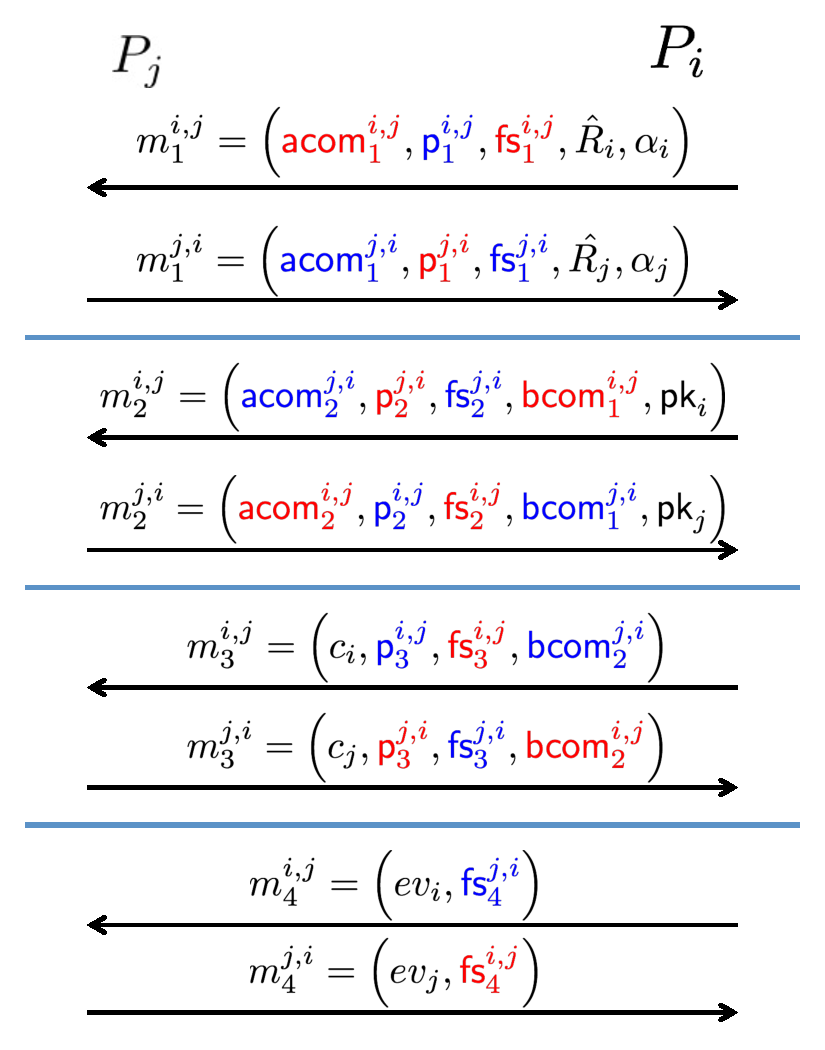
\includegraphics[width=2.8in,height=3.2in]{msg.pdf}}}
\caption{Messages exchanged between party $P_i$ and $P_j$ in $\Pi_\PC$.
  $(\nm_1,\nm_2)$ and $(\onm_1,\onm_2)$ are commitments, $(\WIPOKmsg_1, \WIPOKmsg_2, \WIPOKmsg_3)$ belong to the 3-round $\Pi_\WIPOK$, $(\FLSmsg_1, \FLSmsg_2, \FLSmsg_3,\FLSmsg_4)$ belong to the 4-round $\Pi_\FLS$, and $(\alpha,\pk,c,ev)$ denote the $\MFHE$ messages. Blue messages are sub-protocols where party $P_i$ is the prover/committer and party $P_j$ is the verifier/receiver, red messages are the opposite.}
\label{messages}
\vspace{-3ex}
\end{figure}\anti{I have to update the colored picture to include the $f_i$}
%\begin{figure}
\begin{center}
\begin{tikzpicture}
[
	xscale	= 1.8,	% to scale horizontally everything but the text
	yscale	= 1.8,	% to scale vertically everything but the text
]
\node (MS1121) [draw = none] at	(-1.5,-3.5) {};
\node (ME1121) [draw = none] at	(-0.5,-3.5) {};
\node (MS1122) [draw = none] at	(-1.5,-4.0) {};
\node (ME1122) [draw = none] at	(-0.5,-4.0) {};
\node (MS1123) [draw = none] at	(-1.5,-4.5) {};
\node (ME1123) [draw = none] at	(-0.5,-4.5) {};
\node (MS1124) [draw = none] at	(-1.5,-5.0) {};
\node (ME1124) [draw = none] at	(-0.5,-5.0) {};

\node (MS1211) [draw = none] at	(1.5,-3.5) {};
\node (ME1211) [draw = none] at	(0.5,-3.5) {};
\node (MS1212) [draw = none] at	(1.5,-4.0) {};
\node (ME1212) [draw = none] at	(0.5,-4.0) {};
\node (MS1213) [draw = none] at	(1.5,-4.5) {};
\node (ME1213) [draw = none] at	(0.5,-4.5) {};
\node (MS1214) [draw = none] at	(1.5,-5.0) {};
\node (ME1214) [draw = none] at	(0.5,-5.0) {};
%\node (K0) [draw = none] at	(-7.5,-5.5) {};
%\node (K1) [draw = none] at	(-6.5,-5.5) {};


\draw (-2,-5.5) -- (2,-5.5) -- (2,-2.6) -- (-2,-2.6) -- (-2,-5.5);
%\draw (-9,-7) -- (-2,-7) -- (-2,-2) -- (-9,-2) -- (-9,-7);

\node (P11) [draw = none] at	(-1,-2.75) {\small $P_1$};

\node (P12) [draw = none] at	(1,-2.75) {\small $P_2$};


%%%%%%%%%%%mmmmm%%%%%%%%%%%%%%%%%%%%

\node (m11) [draw = none] at	(-1,-3.425) {\small $m_1$};

\node (m12) [draw = none] at	(-1,-3.925) {\small $\tld{m}_2$};

\node (m13) [draw = none] at	(-1,-4.425) {\small $m_3$};

\node (m14) [draw = none] at	(-1,-4.925) {\small $\tld{m}_4$};

\node (m21) [draw = none] at	(1,-3.425) {\small $\tld{m}_1$};

\node (m22) [draw = none] at	(1,-3.925) {\small $m_2$};

\node (m23) [draw = none] at	(1,-4.425) {\small $\tld{m}_3$};

\node (m24) [draw = none] at	(1,-4.925) {\small $m_4$};
\draw
[
thick,
->
]
(MS1121) to (ME1121);
\draw
[
thick,
->
]
(MS1122) to (ME1122);
\draw
[
thick,
->
]
(MS1123) to (ME1123);
\draw
[
thick,
->
]
(MS1124) to (ME1124);

%%%%OTHER DIRECTION CASE-1%%%%%
\draw
[
thick,
->
]
(MS1211) to (ME1211);
\draw
[
thick,
->
]
(MS1212) to (ME1212);
\draw
[
thick,
->
]
(MS1213) to (ME1213);
\draw
[
thick,
->
]
(MS1214) to (ME1214);

%\node (empty) [draw=none] at (-3.5,-3.25) {$\stackrel{\footnotesize Rescheduled}{\large{\implies}}$};

%%%%%%%%%%%%%%Rounds%%%%%%%%%%%%%

\draw
[
dashed,
]
(-1.75,-3.75) to (1.75,-3.75);

\draw
[
dashed,
]
(-1.75,-4.25) to (1.75,-4.25);

\draw
[
dashed,
]
(-1.75,-4.75) to (1.75,-4.75);




\end{tikzpicture}
\end{center}
\caption{2-PC in the simultaneous message exchange model.}
\label{fig:2-PC}
\end{figure}

%%%%%%%%%%%%%%%%%%%%%%%%%%%%%%












% !TEX root =../main-optimal.tex
%%%%%%%%%%%%%%%%%%%%%%%%%%%%%%%%%%%%%%%%%%%%%%%%%%%%%%%%%%%%%%%%%%%%%%
\subsection{Proof of Security} \label{sec:secProof}
%%%%%%%%%%%%%%%%%%%%%%%%%%%%%%%%%%%%%%%%%%%%%%%%%%%%%%%%%%%%%%%%%%%%%%
\BT 
%Let $\ell_{in}, \ell_{out} \in \NN$ and let $F : (\bit^{\ell_{in}})^N \rightarrow \bit^{\ell_{out}}$ be any deterministic polynomial-time $N$-party functionality. 
Assuming sub-exponential hardness of $\LWE$, and the existence of an adaptively-secure commitment scheme, there exists a four-broadcast-round protocol for securely realizing any functionality against malicious adversary in the plain model with no setup.
\label{thm:main}
\ET

To prove \thmref{main}, we note that the two assumptions listed suffice for instantiating all the components of our protocol $\Pi_{\PC}$: The commitment is used directly for $\nmCom$ and $\Com$, and sub-exponential LWE suffices for everything else.
%\anti{make the theorem nicer}
%
Below we prove security of $\Pi_{\PC}$ by describing a simulator and proving that the simulated view is indistinguishable from the real one.

\subsubsection{Description of the Simulator}\label{sec:simu}

Let $\cA$ be a malicious, static adversary that interacts with parties running the protocol $\Pi_\PC$ from Figure \ref{MPC} in the plain model. We construct a simulator $\cS$ (the ideal world adversary) with access to the ideal functionality $\mathbf{\func}$, which simulates a real execution of $\Pi_\PC$ with $\cA$ such that the ideal world experiment with $\cS$ and $\mathbf{\func}$ is indistinguishable from a real execution of $\Pi_\PC$ with $\cA$. Our simulator $\cS$ proceeds as follows:



\paragraph{Simulating actual protocol messages in $\Pi$:} Let $\ccP = \{P_1,\ldots, P_N\}$ be the set of parties participating in the execution of $\Pi_\PC$. Also let $\ccP^* \subseteq \ccP$ be the set of parties corrupted by the adversary $\cA$. The simulator $\cS$ only generates messages on behalf of parties $\ccP\backslash \ccP^*$. %Without loss of generality we assume that only one party is honest, denoted by $P_h$.


\paragraph{Round 1 Messages $\cS \rightarrow \cA$:} In the first round $\cS$ generates messages on behalf of each honest party $P_h \notin \ccP^*$, as follows:

\BE
\item Choose randomness $r_h=(r^{gen}_h,r^{enc}_h)$ for the $\MFHE$ protocol and an unrelated $\kappa$-bit randomness value~$R_h$, and set $\hat{R}_h=OWF(R_h)$.

\item For every $j$ engage in a two-round commitment protocol with $P_j$. To this end, prepare the first message $\nm_1^{h,j}$ corresponding to the execution of $\nmCom_{\id_j}(x_j,r^{gen}_j,r^{enc}_j,R_j;\omega_{j})$ on behalf of $P_h$, acting as the receiver of the commitment.  Since the commitment $\nmCom$ is a two-round protocol, the message of the committer $P_j$ is only sent in the second round. 

\item Prepare the first message $\WIPOKmsg^{h,j}_1$ of $\Pi_\WIPOK$, where $P_h$ acts as the Prover, for the $\NP$-Language $\hhstPOK$ and the first message $\FLSmsg^{h,j}_1$ of $\Pi_\FLS$ where $P_h$ acts as the Verifier for $\stFLSS$. 

\item Honestly generate the message $\alpha_h$ of the $1$-round protocol $\sf \Pi_{GenSetup}$.

\item It then sends the message $m^{h,j}_1=\left(\hat{R}_h, \nm_1^{h,j}, \WIPOKmsg_1^{h,j},\FLSmsg_1^{h,j},\alpha_h\right)$
 to $\cA$.
\EE

     
     

\paragraph{Round 1 Messages $\cA \rightarrow \cS$:} Also in the first round the adversary $\cA$ generates the messages $m^{j,h}_1=\left(\hat{R}_j, \nm_1^{j,h}, \WIPOKmsg_1^{j,h},\FLSmsg_1^{j,h},\alpha_j\right)$ on behalf of corrupted parties $j\in\ccP^*$ to honest parties $h\notin\ccP^*$. Messages $\{\nm_1^{j,h}\}$ correspond to an execution of $\nmCom_{\id_h}({\bf 0};\omega_{h})$.



\paragraph{Round 2 Messages $\cS \rightarrow \cA$:}  In the second round $\cS$ generates messages on behalf of each honest party $P_h\in \ccP^*$ as follows:

\BE 
\item Complete the commitment to the zero string generating the second messages $\nm_2^{j,h}$ corresponding to all executions of $\nmCom_{\id_h}({\bf 0};\omega_{h})$.

\item Honestly prepare the second message $\WIPOKmsg_2^{j,h}$ ($\FLSmsg_2^{j,h}$) of $\Pi_\WIPOK$($\Pi_\FLS$) initiated by $P_j$ acting as the prover (verifier) in the first round. 

\item Generate the second commitment messages $\onm_1^{h,j}$ for $\Com_{\id_j}({\bf 0};\zeta_j)$ where party $P_h$ acts as the Receiver.

\item Generate the individual key pair by locally computing the matrix~$A$ (on input $\{\alpha_i\}_{i\in[N]}$), and by  computing $(\pk_h, \sk_h) = \Keygen(\params, A;r^{gen}_h)$.

\item It then sends the message $m^{h,j}_2:=(\nm^{j,h}_2, \onm^{h,j}_1, \WIPOKmsg^{j,h}_2, \FLSmsg^{j,h}_2,\pk_h)$ to $\cA$.
\EE


\paragraph{Round 2 Messages $\cA \rightarrow \cS$:} In the second round the adversary $\cA$ generates the messages $m^{j,h}_2:=(\nm^{h,j}_2, \onm^{j,h}_1, \WIPOKmsg^{h,j}_2, \FLSmsg^{h,j}_2,\pk_j)$ on behalf of corrupted parties $j\in\ccP^*$ to honest parties $h\notin\ccP^*$. Messages $\{\nm^{h,j}_2\}$ correspond to an execution of $\nmCom_{\id_j}(x_j,r^{gen}_j,r^{enc}_j,R_j;\omega_{j})$ and messages $\{\onm^{j,h}_1\}$ correspond to an execution of $\Com_{\id_h}({\bf 0};\zeta_{h})$


\paragraph{Round 3 Messages $\cS \rightarrow \cA$:}  In the third round $\cS$ generates messages on behalf of each honest party $P_h\notin\ccP^*$ as follows:

\BE
\item Generate the second messages $\onm_2^{j,h}$ corresponding to all $\Com_{\id_h}({\bf 0};\zeta_h)$. 

\item Generate an encryption of the zero string using randomness $r^{enc}_h$, i.e.  $c_h=\Encrypt(pk_h,{\bf 0};r^{enc}_h)$.

\item Honestly prepare the final message $\WIPOKmsg_3^{h,j}$ ($\FLSmsg_3^{h,j}$) of $\Pi_\WIPOK$($\Pi_\FLS$) initiated by $P_h$ acting as the prover (verifier) in the first round. 

\item It sends the message $m^{h,j}_3=(\onm^{j,h}_2,c_h, \WIPOKmsg^{h,j}_3,\FLSmsg^{h,j}_3)$ to $\cA$.
\EE

\paragraph{Round 3 Messages $\cA \rightarrow \cS$:} In the third round $\cA$ generates $m^{j,h}_3=(\onm^{h,j}_2,c_j, \WIPOKmsg^{j,h}_3,\FLSmsg^{j,h}_3)$ where messages $\{\onm^{h,j}_2\}$ correspond to an execution of $\Com_{\id_j}({\bf 0};\zeta_{j})$.
Then, $\cS$ proceeds to extract the witness corresponding to each proof-of-knowledge completed in the first three rounds (via rewinding). To this end, $\cS$ applies the knowledge extractor of $\Pi_\WIPOK$ to obtain the ``witnesses'' which consist of the inputs and secret keys of the corrupted parties $(x_{j},r_j)$\footnote{For simplicity of exposition, we omit the rest of the witness values.} and the zero knowledge simulator of $\Pi_\FLS$ to obtain the ``trapdoors'' (which for a Feige-Shamir protocol means extracting the verifier-secret). If extraction fails, $\cS$ outputs $\mathsf{fail}$. Next $\cS$ sends $\{x_j\}_{j\in[N]\setminus{\{h\}}}$ to the ideal functionality $\mathbf{\func}$ which responds by sending back $y$ such that $y = F(\{x_j\}_{j \in [N]})$.


\paragraph{Round 4 Messages $\cS \rightarrow \cA$:}  In the fourth round $\cS$ generates messages on behalf of each honest party $P_h\notin\ccP^*$ as follows:
\BE
\item Generate the evaluated ciphertext $\hc:= \Evall(\params; F; (c_1,\ldots, c_N))$.
\item Then, $\cS$ obtains all the secret keys $\{\sk_j\}_{j\in\ccP^*}$ reconstructed from the wintesses $\{r^{gen}_j\}_{j\in\ccP^*}$ and computes the simulated decryption shares $\{ev_h\}_{h\notin\ccP^*}\leftarrow \cS^T(y, \hc,h,\{\sk_j\}{_{j\in\ccP^*}})$. (The simulator $\cS^T$ is the one provided by \cite[Section~6.2]{MW16}.)
\item Fake the final message $\FLSmsg^{j,h}_4$ of $\Pi_\FLS$ protocol using the extracted trapdoor.
It sends the message $m^{h,j}_4=(ev_h, \FLSmsg^{j,h}_4)$ on behalf of $P_h$. 
\EE



\paragraph{Round 4 Messages $\cA \rightarrow \cS$:} In the last round the adversary $\cA$ generates the messages on behalf of corrupted parties in $\ccP^*$. For each party $j\in\ccP^*$ our simulator receives messages ${m}^{j,h}_4=({ev}_j, \tFLSmsg^{h,j}_4)$ from $\cA$.

This completes the description of the simulator.







%%%%%%%%%%%%%%%%%%%%%%%%%%%%%%%%%%%%%%%%%%%%%%%%%%%%%%%%%%%%%%%%%%%%%%%%%%%%
\subsubsection{Proof of Indistinguishability}
We need to prove that for any malicious (static) adversary $\cA$, the view generated by the simulator $\cS$ above is indistinguishable from the real view, namely:
$$
\left\{\ideall_{\mathbf{\func},\cS}(\kappa,\cdot)\right\}_{\kappa} \indist
\left\{\reall_{\Pi,\cA}(\kappa,\cdot)\right\}_{\kappa}
$$
To prove indistinguishability, we consider a sequence of hybrid experiments $H_0,H_1,\ldots$ as described below. Let $H_0$ be the hybrid describing the real-world execution of the protocol. We modify this game in steps as follows:

\begin{itemize}
\item[$H_1$] Use the zero-knowledge simulator to generate the proof in the $4$-round $\Pi_{\FLS}$, indistinguishability follows by the ZK property of $\Pi_{\FLS}$.
\item[$H_2$] Starting in this hybrid, the challenger is given access to a breaking oracle $\calB_{\tagg}$ (with $\tagg=(\id_h,\star)$ where $h$ is a honest party). Here the challenger uses the breaking oracle to extract the values committed to by the adversary in $\nm_2^{h,\cA}$ (in the second round), then commits to these same values in $\onm_2^{\cA,h}$ on behalf of the honest party (in the third round). Indistinguishability follows by the adaptive-hiding of $\Com$.

\item[$H_3$] Change the proof in $\Pi_{\WIPOK}$ to use the ``OR branch''. Indistinguishability follows by the WI property of $\Pi_{\WIPOK}$ (which must hold even in the presence of the breaking-oracle $\calB_{\tagg}$). 

\item[$H_4$] Here the challenger also has access to the ideal-world functionality that gives it the output of the function. Having extracted the secret keys using $\calB_{\tagg}$, the challenger \emph{simulates the decryption shares} of the honest parties rather than using the decryption procedure.
  Indistinguishability follows since the FHE scheme is simulatable (which follows from $\LWE$).

\item[$H_5$] Encrypt $0$'s rather than the true inputs. Indistinguishability follows due to the semantic security of the encryption scheme (that follows from the ILWE-hardness of our scheme, under LWE).

\item[$H_6$] Commit to $0$'s in $\nm_2^{\cA,h}$, rather than to the real inputs. Indistinguishable due to the adaptive-hiding of $\nmCom$.

\item[$H_7$] Revert the change in $H_3$, make the proof in $\Pi_{\WIPOK}$ use the normal branch rather than the ``OR branch''. Indistinguishability follows by the WI property of $\Pi_{\WIPOK}$.

\item[$H_8$] Revert the change in $H_2$ and thus commit to zero in $\onm_2^{\cA,h}$ (instead of committing to the extracted values).  Indistinguishability follows by the adaptive-hiding of $\Com$.

\item[$H_9$] Here the challenger no longer has access to a breaking oracle, and instead it uses the POK extractor to get the randomness and inputs (witnesses) from $\Pi_{\WIPOK}$. Indistinguishability follows from the extraction property of $\Pi_{\WIPOK}$, combined with the one-wayness of $OWF$.
\end{itemize}
As $H_9$ we no longer uses the inputs of the honest parties, the view of this hybrid can be simulated. (We also note that the simulator \emph{does not use a breaking oracle}, rather it is a traditional rewinding simulator.)


\paragraph{Security in the presence of a breaking oracle:}
Note that some of our indistinguishability arguments must holds in worlds with a breaking oracle $\calB_{\tagg}$. In particular, we require that $\Com$ is still hiding, that LWE still holds, and that $\Pi_{\WIPOK}$ is still witness-indistinguishable in the presence of the oracle. The hiding property of $\Com$ follows directly from its adaptive-hiding property. As for LWE and $\Pi_{\WIPOK}$, security in the presence of $\calB_{\tagg}$ follows from sub-exponential hardness and complexity leveraging. Namely, in the relevant reductions we can implement $\calB_{\tagg}$ ourselves in subexponential time, while still relying on the hardness of LWE or $\Pi_{\WIPOK}$.

Another point to note is that using the zero-knowledge simulator (in hybrids $H_2$-$H_9$) requires rewinding, which may be problematic when doing other reductions. As we explain below, we are able to handle rewinding by introducing many sub-hybrids, essentially cutting the distinguishing advantage by a factor equals to the number of rewinding operations.


\BDE
\item{$\bf H_0$:} This hybrid is the real execution. In particular, $H_0$ starts the execution of $\cA$ providing it fresh randomness and input $\{x_j\}_{P_j \in\ccP^* }$, and interacts with it honestly by performing all actions of the honest parties with uniform randomness and input. The output consists of $\cA$'s view.


\smallskip
\item{$\bf H_1$:} In this hybrid the challenger uses the zero-knowledge simulator of $\Pi_{\FLS}$ to generate the proofs on behalf of each honest party~$\P_h$, rather than the honest prover strategy as is done in ${\bf H_0}$.
  We note that the challenger in this hybrid needs to rewind the adversary $\cA$ (up to the second round) as needed for the Feige-Shamir ZK simulator.

  Since in these two hybrids the protocol $\Pi_{\FLS}$ is used to prove the same true statement, then the simulated proofs are indistinguishable from the real ones, so we get:
  
\BL $\Hyb{0} \statind  \Hyb{1}$.\EL


\smallskip
\item{$\bf H_2$:} In this ``mental-experiment hybrid'' the challenger is given access to a breaking oracle $\calB_{\id_h}$, with the tag being the identity of an arbitrary honest parties ($h\notin\ccP^*$).
  The challenger begins as in the real execution for the first two rounds, but then it uses $\calB_{\tagg}$ to extract the values $(x_j,r_j,R_j)$ of all the adversarial players $j\in\ccP^*$ from $\nm_2^{h,j}$.

  Then the challenger changes the commitments $\onm_2^{j,h}$ on behalf of the honest party $P_h$, committing to the values $R_j$ that were extracted from $\nm_2^{h,j}$ (and thus making the language $\hhtwost$~--the ``OR branch''--~in $\Pi_{\WIPOK}$ a true statement).%
\footnote{The commitment $Com$ starts in the second round, but this is a two-round commitment so the committed value only affects the second message in the commitment, which happens in the third round of the larger protocol.}

\BL\label{lemmab}$\Hyb{1} \compind  \Hyb{2}$.\EL
\begin{proof}
Since the only differences between these hybrids are the values committed to in $\onm^{j,h}$, then indistinguishability should follow from the adaptive-hiding of the commitment scheme $\Com$ (as the challenger never queries its breaking oracle with any tag containing the identity $\id_h$ of the honest party).

One subtle point here, is that in both $\Hyb{1}$ and $\Hyb{2}$ we use the rewinding Feige-Shamir ZK simulator, so we need to explain how the single value $\onm_2^{j,h}$ provided by the committer in the reduction (which is a commitment to either $0$ or $R_j$) is used in all these transcripts. To that end let $M$ be some polynomial upper bound on the number of rewinding operations needed by the zero-knowledge simulator. The reduction to the security of~$\Com$ will choose at random $t\in[1,M]$ and will only use the $\Com$ committer that it interacts with to commit to a value in the $t$'th rewinding, committing to $0$ in all the rewindings $i<t$ and to the value $R_j$ (that it has from the breaking oracle) in all the rewindings $i>t$.

By a standard argument, if we can distinguish between $\Hyb{1} \compind  \Hyb{2}$ with probability $\epsilon$ then the reduction algorithm can distinguish commitments to 0 and $R_j$ with probability $\epsilon/M$.
\end{proof}

\smallskip
\item{$\bf H_3$:} In this hybrid, we change the witness used in $\Pi_\WIPOK$ on behalf of each honest party $P_h$. In particular, all $\Pi_\WIPOK$ executions use the ``OR branch'' $\hhtwost$.

\BL\label{wipok}$\Hyb{2} \compind  \Hyb{3}$.\EL

\begin{proof}
We make sub-hybrids that change one honest party at a time, and show that a distinguisher $D$ that distinguishes two such sub-hybrids can be used by another distinguisher $D'$ to distinguish between the two witnesses of $\Pi_{WIPOK}$ (as per \defref{dWI}).

%%%%%%%%%%%%%%%%%%%%%%%%%%%%%%%%%%%%%
{\bf Description of $D'$}: $D'$ plays the role of both the challenger and the adversary in the two hybrids, except that the prover messages of $\Pi_\WIPOK$ (on behalf of $P_h$) are obtained from the external prover that the WI-distinguisher $D'$ has access to.

At the third round of the protocol, $D'$ has the statement that $P_h$ needs to prove, and it gets the two witnesses for that statement from the witness-selecting machine in \defref{dWI}. Sending the statement and witnesses to its external prover, $D'$ obtains the relevant $\Pi_\WIPOK$ message (for one of them). $D'$ also uses these witnesses to complete the other flows of the protocol (e.g., the commitments $\onm_2^{j,h}$ that include some of these witnesses). Once the protocol run is finished, it gives the transcript to $D$ and outputs whatever $D$ outputs.

As above, we still need to support rewinding by the Feige-Shamir ZK simulator, while having access to only a single interaction with the external prover, and we do it by sub-sub-hybrids where we embed this interaction in a random rewinding~$t$, producing all the other proofs by the $H_2$ challenger (for $i<t$) or the $H_3$ challenger (for $i>t$). It is clear that the advantage of $D'$ is a $1/M$ fraction of the advantage of~$D$.
\end{proof}

\medskip
We note that $D'$ above still uses the breaking oracle $\calB_{\tagg}$ (to extract the $\Pi_{\FLS}$ secrets), so we need to assume that delayed-input-WI holds even in a world with the breaking oracle. As explained above, we rely on complexity leveraging for that purpose. That is, we let $D'$ run in subexponential time (so it can implement $\calB_{\tagg}$ itself), and set the parameters of $\Pi_\WIPOK$ large enough so we can assume witness-indistinguishability even for such a strong~$D'$. (We can implement subexponential WI protocol from subexponential LWE.)

\smallskip
%%%%%%
\item{$\bf H_4$:} The difference from $H_3$ is that in $H_4$ we simulate the decryption shares of the honest parties. More specifically, the challenger in $H_4$ has access also to the ideal functionality, and it proceeds as follows:
\BE
\item It completes the first three broadcast rounds exactly as in $H_3$.

\item Having extracted the input of all the corrupted parties, the challenger sends all these inputs to the ideal functionality $\mathbf{\func}$ and receives back the output $y = F(\{x_j\}_{j \in [N]})$.

\item Having extracted also all the secret keys of the corrupted parties, the challenger has everything that it needs to compute the simulated decryption shares of the honest parties, $\{ev_h\}_{h\notin\ccP^*}\leftarrow \cS^T(y, \hc,h,\{\sk_j\}{_{j\in\ccP^*}})$.

\item The challenger computes also the last message of $\Pi_{\FLS}$ (using the simulator as before), and sends it together with decryption shares $\{ev_h\}_h$ in the last round.
\EE

%%%%%
\BL$\Hyb{3} \statind  \Hyb{4}$.\EL
\begin{proof}
  The only change between these two experiments is that the partial decryption shares of the honest parties are not generated by partial decryption. Instead they are generated via the the threshold simulator $\cS^T$ of the $\MFHE$ scheme. By the simulatability of threshold decryption, the partial decryptions shares are statistically indistinguishable.
\end{proof}


\smallskip
\item{$\bf H_5$:} 
We change $H_4$ by making $\cS$ broadcast encryptions of ${\bf 0}$ on behalf of the honest parties in the third round, instead of encrypting the real inputs. 
\smallskip
\BL$\Hyb{4} \compind  \Hyb{5}$.
\label{lem:Hyb5-6}
\EL
\begin{proof}
The proof follows directly from semantic security, which in our case follows from LWE. As in the previous hybrid, here too we need this assumption to hold even in the presence of a breaking oracle, and we lose a factor of $M$ in the distinguishing probability due to rewinding.
\end{proof}

\smallskip
\item{$\bf H_6$:} In this hybrid, we get rid of the honest partys' inputs $\{(x_h,r_h)\}_h$ (that are present in the values of $\nm_2^{j,h}$). Formally, $H_6$ is identical to $H_5$ except that in the first round it sets $x_h={\bf 0}$ for all $h\notin\ccP^*$.

\BL$\Hyb{5} \compind  \Hyb{6}$.\EL

\begin{proof}
  This proof is very similar to the the proof of $\Hyb{1} \compind  \Hyb{2}$, and indistinguishability follows from adaptive-hiding of $\nmCom$. Since the challenger never asks its breaking oracle $\calB_{\tagg}$ to break commitments relative to the honest party's tags (and since these committed values are no longer used by the challenger for anything else), then having the honest parties commit to $x_h$ is indistinguishable from having it commit to ${\bf 0}$.
\end{proof}

\smallskip
\item{$\bf H_7$:} In this hybrid we essentially reverse the change that was made in going from $H_2$ to $H_3$. Namely, since now both the encryption and the commitment at each honest party are for the value ${\bf 0}$ then there is no need to use the ``OR branch'' in $\Pi_{\WIPOK}$. Hence we return in using the honest prover strategy there, relative to the input $x_h=0$. As in Lemma \ref{wipok} indistinguishability follows by the WI property of $\Pi_{\WIPOK}$. 

\smallskip
\item{$\bf H_{8}$:} Revert the change that was made in going from $H_1$ to $H_2$ and thus commit to a random value $s_h$ in $\onm_2^{j,h}$.  Indistinguishability follows by the computational hiding of $\Com$, just like in Lemma \ref{lemmab}.

\smallskip
\item{$\bf H_{9}$:} In this hybrid the challenger no longer has access to the breaking oracle $\calB_{\tagg}$. Instead, it uses the knowledge extractor of $\Pi_{\WIPOK}$ to get the input and secret keys of the corrupted parties, and the ``standard'' zero-knowledge simulator to get the proof in $\Pi_{\FLS}$.

\BL$\Hyb{8} \statind  \Hyb{9}$.\EL

\begin{proof}
  The only difference between these hybrids is the method used by the challenger to extract the adversary secrets. Two technical points needs to be addressed here:
  \begin{itemize}
  \item
    This hybrid requires rewinding by \emph{both} the FS ZK simulator and the FLS knowledge extractor, so we need to argue that after polynomially many trials they will \emph{both succeed} on the same transcript. This is a rather standard argument (which essentially boils down to looking at the knowledge-extractor inside $\Pi_{\FLS}$ and the one used explicitly in $\Pi_{\WIPOK}$ as extracting knowledge for and AND language.)

  \item
    We also need to argue that the value extracted from the adversary by the $\Pi_{\WIPOK}$ extractor in $\Hyb{9}$ is a witness for $\onest$ and not for $\twost$. This is done by appealing to the one-wayness of $OWF$, if there is a noticeable probability to extract an $\twost$ witness in $H_9$ then we get an inverter for this one-way function.
  \end{itemize}
  We conclude that in both $\Hyb{8}$ and $\Hyb{9}$ we succeed in extraction with about the same probability, and moreover extract the very same thing, and (statistical) indistinguishability follows.
\end{proof}
\EDE
We conclude the proof by observing that the hybrid $H_9$ is identical to the ideal-world game with the simulator.
\qed



\bibliographystyle{alpha}
\bibliography{abbrev3,refs,crypto,extra}

\appendix
% !TEX root =../main-optimal.tex

% !TEX root =../main-optimal.tex

% !TEX root =../main-optimal.tex		--- NOT TRUE ANYMORE
% % !TEX root =./appendix.tex

\section{Secure Computation Definitions}
\label{sec:mpc}

For completeness, we recall the definition of secure computation based on \cite[Chapter 7]{Goldreich04} here. We only recall the two party case as it is most relevant to our proofs. The description naturally extends to multi-party case as well (details can be found in \cite{Goldreich04}).


\paragraph{Two-party computation.} A two-party protocol problem is cast by specifying a random process
that maps pairs of inputs to pairs of outputs (one for each party). We refer to such a process as
a functionality and denote it $\mathbf{\func} : \bit^* \times \bit^*\rightarrow\bit^* \times \bit^*$ where $\mathbf{\func} = (F_1, F_2)$. That is,
for every pair of inputs $(x, y)$, the output-pair is a random variable $(F_1(x, y), F_2(x, y))$ ranging over
pairs of strings. The first party (with input $x$) wishes to obtain $F_1(x, y)$ and the second party (with
input $y$) wishes to obtain $F_2(x, y)$.


\paragraph{Adversarial behavior.} Loosely speaking, the aim of a secure two-party protocol is to protect
an honest party against dishonest behavior by the other party. In this paper, we consider malicious
adversaries who may arbitrarily deviate from the specified protocol. When considering malicious
adversaries, there are certain undesirable actions that cannot be prevented. Specifically, a party
may refuse to participate in the protocol, may substitute its local input (and use instead a different
input) and may abort the protocol prematurely. One ramification of the adversary's ability to
abort, is that it is impossible to achieve {\em fairness}. That is, the adversary may obtain its output
while the honest party does not. In this work we consider a static corruption model, where one of the parties is adversarial and the other is honest, and this is fixed before the execution begins.


\paragraph{Communication channel.} In our results we consider a secure simultaneous message exchange channel in which all parties can simultaneously send messages over the channel at the same communication round. Moreover, we assume an asynchronous network\footnote{The fact that the network is asynchronous means that the messages are not necessarily delivered in the order which
they are sent.} where the communication is open (i.e. all the communication between the parties is seen by the adversary) and delivery of messages is not guaranteed. For simplicity, we assume that the delivered messages are authenticated. This can be achieved using standard methods.



\paragraph{Security of protocols (informal).} The security of a protocol is analyzed by comparing what an
adversary can do in the protocol to what it can do in an ideal scenario that is secure by definition.
This is formalized by considering an ideal computation involving an incorruptible trusted third
party to whom the parties send their inputs. The trusted party computes the functionality on the
inputs and returns to each party its respective output. Loosely speaking, a protocol is secure if
any adversary interacting in the real protocol (where no trusted third party exists) can do no more
harm than if it was involved in the above-described ideal computation.



\paragraph{Execution in the ideal model. } As we have mentioned, some malicious behavior cannot be
prevented (for example, early aborting). This behavior is therefore incorporated into the ideal
model. An ideal execution proceeds as follows:
\BDE
\item {\bf Inputs:} Each party obtains an input, denoted $w$ ($w = x$ for $\sen$, and $w = y$ for $\rec$).
\item  {\bf Send inputs to trusted party:} An honest party always sends $w$ to the trusted party. A malicious
party may, depending on $w$, either abort or send some $w' \in\bit^{|w|}$ to the trusted party.
\item  {\bf Trusted party answers first party:} In case it has obtained an input pair $(x, y)$, the trusted
party first replies to the first party with $F_1(x, y)$. Otherwise (i.e., in case it receives only one
valid input), the trusted party replies to both parties with a special symbol $\bot$.
\item  {\bf Trusted party answers second party: } In case the first party is malicious it may, depending on
its input and the trusted party's answer, decide to stop the trusted party by sending it $\bot$ after
receiving its output. In this case the trusted party sends $\bot$ to the second party. Otherwise
(i.e., if not stopped), the trusted party sends $F_2(x, y)$ to the second party.
\item  {\bf Outputs:} An honest party always outputs the message it has obtained from the trusted party. A
malicious party may output an arbitrary (probabilistic polynomial-time computable) function
of its initial input and the message obtained from the trusted party.
\EDE
Let $\mathbf{\func} : \bit^* \times \bit^*\rightarrow\bit^* \times \bit^*$ be a functionality where $\mathbf{\func} = (F_1, F_2)$ and let $\cS =
(\cS_1, \cS_2)$ be a pair of non-uniform probabilistic expected polynomial-time machines (representing
parties in the ideal model). Such a pair is {\em admissible} if for at least one $i\in \{1, 2\}$ we have that $\cS_i$
is honest (i.e., follows the honest party instructions in the above-described ideal execution). Then,
the {\em joint execution of $F$ under $\cS$ in the  ideal model} (on input pair $(x, y)$ and security parameter $\kappa$), denoted $\ideall_{\mathbf{\func},\cS}(\kappa,x,y)$
is defined as the output pair of $\cS_1$ and $\cS_2$ from the above ideal execution.


\paragraph{Execution in the real model.} We next consider the real model in which a real (two-party)
protocol is executed (and there exists no trusted third party). In this case, a malicious party
may follow an arbitrary feasible strategy; that is, any strategy implementable by non-uniform
probabilistic polynomial-time machines. In particular, the malicious party may abort the execution
at any point in time (and when this happens prematurely, the other party is left with no output).
Let $\mathbf{\func}$ be as above and let $\Pi$ be a two-party protocol for computing $\mathbf{\func}$. Furthermore, let $\cA =
(\cA_1, \cA_2)$ be a pair of non-uniform probabilistic polynomial-time machines (representing parties in
the real model). Such a pair is {\em admissible} if for at least one $i \in \{1, 2\}$ we have that $\cA_i$
is honest (i.e., follows the strategy specified by $\Pi$). Then, the {\em joint execution of $\Pi$ under $\cA$ in the real model}, denoted $\reall_{\Pi,\cA}(\kappa,x,y)$, is defined as the output pair of $\cA_1$ and $\cA_2$ resulting
from the protocol interaction.

\paragraph{Security as emulation of a real execution in the ideal model.} Having defined the ideal
and real models, we can now define security of protocols. Loosely speaking, the definition asserts
that a secure two-party protocol (in the real model) emulates the ideal model (in which a trusted
party exists). This is formulated by saying that admissible pairs in the ideal model are able to
simulate admissible pairs in an execution of a secure real-model protocol.



\BD[secure two-party computation] Let $\mathbf{\func}$ and $\Pi$ be as above. Protocol $\Pi$ is said to
securely compute $\mathbf{\func}$ (in the malicious model) if for every pair of admissible non-uniform probabilistic
polynomial-time machines $\cA =
(\cA_1, \cA_2)$ for the real model, there exists a pair of admissible non-uniform
probabilistic expected polynomial-time machines $\cS =(\cS_1, \cS_2)$  for the ideal model, such that:

$$
\left\{\ideall_{\mathbf{\func},\cS}(\kappa,x,y)\right\}_{\kappa\in\NN,x,y ~{\text  s.t. } ~|x|=|y|} \indist
\left\{\reall_{\Pi,\cA}(\kappa,x,y)\right\}_{\kappa\in\NN,x,y ~{\text  s.t. } ~|x|=|y|}
$$

%Namely, the two distributions are computationally indistinguishable.
\ED

We note that the above definition assumes that the parties know the input lengths (this can be
seen from the requirement that $|x| = |y|$). Some restriction on the input lengths is unavoidable,
see \cite[Section 7.1]{Goldreich04} for discussion. We also note that we allow the ideal adversary/simulator to
run in expected (rather than strict) polynomial-time. This is essential for constant-round
protocols \cite{BL04}.
%We denote the security parameter by $\kappa$ and, for the sake of simplicity, unify it with the length
%of the inputs (thus we consider security for ``all sufficiently long inputs''). 

%The above naturally extends to the multi-party computation setting. 
\remove{\section{General Definitions}
\subsection{Witness Relations}

We recall the definition of a witness relation for an NP language \cite{Goldbook,STOC:LinPas11}.
\BD[Witness relation] A \emph{witness relation} for a language $L \in \NP$ is a binary relation
$R_L$ that is polynomially bounded, polynomial time recognizable and characterizes $L$ by $L = \{x: ~\exists~ y ~\text{s.t.} ~(x,y)\in R_L\}$
\ED
We say that $y$ is a witness for the membership $x \in L$ if  $(x,y)\in R_L$. We will also let $R_L(x)$
denote the set of witnesses for the membership $x \in L$, i.e., $R_L(x) = \{y:(x,y)\in L \}$. In the
following, we assume a fixed witness relation $R_L$ for each language $L \in \NP$.

\subsection{Interactive Proofs}
%We use the standard definitions of interactive proofs (and interactive Turing machines) [GMR89]
%and arguments (a.k.a. computationally-sound proofs) [BCC88]. 

Given a pair of interactive Turing
machines, $P$ and $V$ , we denote by $\langle P(w), V \rangle(x)$ the random variable representing the (local) output
of $V$, on common input $x$, when interacting with machine $P$ with private input $w$, when the random
input to each machine is uniformly and independently chosen.

\BD [Interactive Proof System] A pair of interactive machines $\langle P, V \rangle$ is called an \emph{interactive proof system} for a language $L$ if there is a negligible function $\mu(\cdot)$ such that the following two conditions hold:
\BI
\item Completeness: For every $x \in L$, and every $w\in R_L(x)$, $Pr [\langle P(w), V \rangle(x)= 1] = 1$. 
\item  Soundness: For every $x \notin L$, and every interactive machine $P^*, Pr [\langle P^*, V \rangle(x) = 1] \leq\mu(\kappa)$
\EI
In case the soundness condition is required to hold only with respect to a computationally
bounded prover, the pair $\langle P, V \rangle$ is called an interactive argument system.
\ED

\subsection{Zero-Knowledge}
We recall the standard definition of ZK proofs. Loosely speaking, an interactive proof is said to be
zero-knowledge (ZK) if a verifier $V$ learns nothing beyond the validity of the assertion being proved,
it could not have generated on its own. As ``feasible''computation in general is defined though
the notion of probabilistic polynomial-time, this notion is formalized by requiring that the output
of every (possibly malicious) verifier interacting with the honest prover $P$ can be ``simulated" by
a probabilistic expected polynomial-time machine $\cS$ (a.k.a. the simulator). The idea behind this
definition is that whatever $V^*$ might have learned from interacting with $P$, he could have learned
by himself by running the simulator $\cS$. 

\BD [ZK]. Let $L$ be a language in $\NP$, $R_L$ a witness relation for $L$, $(P,V )$ an interactive
proof (argument) system for $L$. We say that $(P, V )$ is \emph{statistical/computational ZK}, if for every
probabilistic polynomial-time interactive machine $V$ there exists a probabilistic algorithm $\cS$ whose
expected running-time is polynomial in the length of its first input, such that the following ensembles
are statistically close/computationally indistinguishable over $L$.
\BI
\item $\{\langle P(y), V(z) \rangle(x)\}_{\kappa\in \NN\,x\in \bit^\kappa\cap L, y \in R_L(x), z\in\bit^*}$
\item $\{\cS (x,z)\}_{\kappa\in \NN\,x\in \bit^\kappa\cap L, y \in R_L(x), z\in\bit^*}$
\EI

where $\langle P(y), V(z) \rangle(x)$ denotes the view of $V$ in interaction with $P$ on common input $x$ and private
inputs $y$ and $z$, respectively.

\ED

\subsection{Witness Indistinguishability}
An interactive proof (or argument) is said to be witness indistinguishable (WI) if the verifier's
output is ``computationally'' independent of the witness used by the prover for proving the statement.
In this context, we focus on languages $L \in \NP$ with a corresponding witness relation $R_L$.
Namely, we consider interactions in which, on common input $x$, the prover is given a witness in
$R_L(x)$. By saying that the output is computationally independent of the witness, we mean that
for any two possible $\NP$-witnesses that could be used by the prover to prove the statement $x \in L$,
the corresponding outputs are computationally indistinguishable.

\BD [Witness-indistinguishability]. Let $\langle P, V \rangle$ be an interactive proof (or argument) sys-
tem for a language $L \in \NP$. We say that $\langle P, V \rangle$ is \emph{witness-indistinguishable} for $R_L$, if for every
probabilistic polynomial-time interactive machine $V^*$ and for every two sequences $\{w^1_{\kappa,x}\}_{\kappa\in \NN,x\in L}$ and $\{w^2_{\kappa,x}\}_{\kappa\in \NN,x\in L}$, such that $w^1_{\kappa,x}, w^2_{\kappa,x}\in R_L(x)$ for every $x \in L\cap \bit^\kappa$, the following probability
ensembles are computationally indistinguishable over $\kappa\in \NN$.
\ED

\BI
\item $\{\langle P(w^1_{\kappa,x}), V^*(z) \rangle(x)\}_{\kappa\in \NN\,x\in \bit^\kappa\cap L, z\in\bit^*}$
\item $\{\langle P(w^2_{\kappa,x}), V^*(z) \rangle(x)\}_{\kappa\in \NN\,x\in \bit^\kappa\cap L, z\in\bit^*}$
\EI
\subsection{Proofs (Arguments) of Knowledge}
Loosely speaking, an interactive proof is a proof of knowledge if the prover convinces the verifier
that it possesses, or can feasibly compute, a witness for the statement proved. The notion of a
proof of knowledge is essentially formalized as follows: an interactive proof of $x \in L$ is a proof of
knowledge if there exists a probabilistic expected polynomial-time extractor machine $E$, such that
for any prover $P$, $E$ on input the description of $P$ and any statement $x \in L$ readily outputs a valid
witness for $x \in L$ if $P$ succeeds in convincing the Verifier that $x \in L$. Formally,

\BD[Proof of knowledge] Let $(P, V )$ be an interactive proof system for the language
$L$. We say that $(P, V )$ is a proof of knowledge for the witness relation $R_L$ for the language $L$ it there
exists an probabilistic expected polynomial-time machine $E$, called the extractor, and a negligible
function $\mu(\cdot)$ such that for every machine $P^*$, every statement $x \in \bit^\kappa$, every random tape
$x \in \bit^*$, and every auxiliary input $z \in \bit^*$,
$$Pr [ \langle P^*_r(z), V \rangle(x) = 1]\leq Pr[E^{P^*_r(x,z)}(x) \in R_L(x)] + \mu(\kappa)$$
\ED

An interactive argument system $\langle P, V \rangle$ is an argument of knowledge if
the above condition holds w.r.t. probabilistic polynomial-time provers.

\paragraph{Special-sound WI proofs.} A $4$-round public-coin interactive proof for the language $L \in \NP$ with
witness relation $R_L$ is special-sound with respect to $R_L$, if for any two transcripts $(\delta,\alpha,\beta, \gamma)$ and $(\delta',\alpha',\beta', \gamma')$ such that the initial two messages, $(\delta,\delta')$ and $(\alpha,\alpha')$ are the same but the challenges $(\beta,\beta')$ are different, there is a deterministic procedure to extract the witness from the two transcripts
and runs in polynomial time. Special-sound WI proofs for languages in $\NP$ can be based on
the existence of $2$-round commitment schemes, which in turn can be based on one-way functions.
%[GMW91, FS90, HILL99, Nao91].
\paragraph{Adaptive-Input Witness Indistinguishability.}
The most recent $3$-round adaptive-Input Witness Indistinguishability we can use appears in the work of \cite{COSV16}. 
The notion of adaptive-input WI formalizes security of the prover with respect to an adversarial
verifier $A$ that adaptively chooses the input instance to the protocol, after seeing the first message of the prover. More specifically, for a delayed-input $3$-round complete protocol , we
consider game ${\sf ExpAWI}$ between a challenger $C$ and an adversary $A$ in which the instance $x$ and
two witnesses $w_0$ and $w_1$ for $x$ are chosen by $A$ after seeing the first message of the protocol played
by the challenger. The challenger then continues the game by randomly selecting one of the two
witnesses and by computing the third message by running the prover's algorithm on input the
instance $x$, the selected witness $w_b$ and the challenge received from the adversary. The adversary
wins the game if she can guess which of the two witnesses was used by the challenger.
The experiment is parameterized by a delayed-input $3$-round complete protocol  $(P, V)$ for a relation $R$ and by a $\ppt$
adversary $A$. The experiment has as input the security parameter and auxiliary information for $A$. 
The experiment ${\sf ExpAWI}$ proceeds as follows: 
\BE
\item $C$ randomly selects coin tosses $r$ and runs P on input $(1^\kappa; r)$ to obtain $a$;
\item $A$, on input $a$ and $aux$, outputs instance $x$, witnesses $w_0$ and $w_1$ such that
$(x,w_0), (x,w_1) \in R$, challenge $c$ and internal state $\sf state$;
\item $C$ randomly selects $b\leftarrow \bit$ and runs $P$ on input $(x,w_b, c)$ to obtain $z$;
\item $b'  \leftarrow A((a, c, z), aux, \sf state)$;
\item if $b = b'$ then output $1$ else output $0$.
\EE
 
\BD[Adaptive-Input Witness Indistinguishability]. A delayed input $3$-round complete
protocol is adaptive-input WI if for any $\ppt$ adversary $A$ there exists a negligible function $\mu(\cdot)$ such that for any $aux \in\bit^*$ it holds that ${\sf AdvAWI}_A(\kappa, aux)\leq \mu(\kappa)$ where ${\sf AdvAWI}_A(\kappa, aux) = |Pr[{\sf AdvAWI}_A(\kappa, aux)=1]-1/2|$
\ED}

%% !TEX root =./main-optimal.tex
\section{Proof Systems}
\label{sec:proofsystems}

We provide a detailed description of the proof systems used in this work.

\subsection{Protocol $\Pi_\WIPOK$} 
This is essentially the Feige-Lapidot-Shamir protocol, slightly reworded in \cite{KatzO04}, mostly for notational convenience.  We recall this protocol here. We denote the messages of this protocol by $(\WIPOKmsg_1, \WIPOKmsg_2,\WIPOKmsg_3)$.

We will be working with the NP-complete language $\it HC$ of graph Hamiltonicity,
and thus assume statements to be proven take the form of graphs,
while witnesses correspond to Hamilton cycles. If $\thmm$ is a graph, we abuse notation
and also let $\thmm$ denote the statement ``$\thmm \in {\it HC}$''. We show how the
proof system can be used to prove the following statement: $\thmm \land \thmm'$, where
$\thmm$ will be included as part of the first message, while $\thmm'$
is only decided in the last round. The
proof system $\Pi_\WIPOK$ runs $\kappa$ parallel executions of the following $3$-round protocol:

\BE

\item The prover commits to two adjacency matrices for two randomly-chosen cycle
graphs $G,G'$. The commitment is done bit-by-bit using a perfectly-binding
commitment scheme.
\item The verifier responds with a single bit $b$, chosen at random.
\item If $b = 0$, the prover opens all commitments. If $b = 1$, the prover sends two
permutations mapping the cycle in $\thmm$ (resp., $\thmm'$) to $G$ (resp., $G'$). For
each non-edge in $\thmm$ (resp., $\thmm'$), the prover opens the commitment at the
corresponding position in $G$ (resp., $G'$).
\item[] The verifier checks that all commitments were opened correctly. If $b = 0$, the
verifier additionally checks whether both decommitted graphs are indeed
cycle graphs. If $b = 1$, the verifier checks whether each non-edge in $\thmm$
(resp., $\thmm'$) corresponds to a non-edge in $G$ (resp., $G'$).
\EE

Note that the prover does not need to know either $\thmm$ or $\thmm'$ (or the corresponding
witnesses) until the beginning of the third round. In the above proof system, we assume that 
$\thmm$ is fixed as part of the first-round message enabling us to
claim stronger properties about the proof system. In particular, $\Pi_\WIPOK$ proof system is complete and sound. More specifically, the probability that an all-powerful
prover can cause a verifier to accept when either $\thmm$ or $\thmm'$
are not true
is at most $2^{-\kappa}$. We stress that this holds even if the prover can adaptively
choose  $\thmm'$ after viewing the second-round message of the verifier. Moreover, $\Pi_\WIPOK$ is witness indistinguishable and it is a proof of knowledge for $\thmm$. (More formally, we can achieve a notion
similar to that of ``witness-extended emulation'' \cite{C:Lindell01} for $\thmm$.) Note also that the first round of the above proof system (as well as the
internal state of the prover immediately following this round) is independent of
$\thmm$ or the associated witness.


\subsection{Protocol $\Pi_\FLS$}\label{sec:fs}

As noted in Section \ref{sec:prelim}, this is essentially the four round zero-knowledge protocol of Feige-Shamir, except that we use {\em non-malleable commitments} in the first three round of the protocol. Following the discussion in Section \ref{sec:prelim}, we let \nmcom\ be a non-malleable commitment scheme, and make the simplifying assumption that \nmcom\ has just three rounds and the first round is committing. Again, these are purely for notational convenience and can easily be removed (as discussed earlier).

We now simply list all the steps of this protocol following \cite{KatzO04}, but using \nmcom. The messages of this protocol are denoted by 
$(\FLSmsg_1, \FLSmsg_2,\FLSmsg_3, \FLSmsg_4)$. It allows the prover to prove $\thmm \land \thmm'$ where  $\thmm$ is sent as part of the second round yet $\thmm'$ is only sent as part of the last round. (Intuitively, statements $\thmm,\thmm'$ will correspond to statements $\st_1,\st_2$ of $\Pi_\WIPOK$ described above.)

The proof system $\Pi_\FLS$ proceeds as follows: 



\BE

\item The first round is as in the original Feige-Shamir protocol but augmented with an $\nmCom$ scheme.  Explicitly, the verifier $V$ selects randomly and independently two values $\sigma_1$ and $\sigma_2$ and computes the first message of two independent executions of $\nmCom$ for $\sigma_1$ and $\sigma_2$, with randomness $\rho_1,\rho_2$ respectively. Let $\nm_1^{\sigma_1}$ and $\nm_2^{\sigma_2}$ be these messages, which $V$ sends to $P$. %corresponding to $\sigma_1$ and $\sigma_2$ respectively. %The transcripts of these executions up to the $\rnm-2$ round are denoted by $\nmCom(\sigma_{1})$ and $\nmCom(\sigma_{2})$, respectively. 

Moreover, $V$ sends the first message $\WIPOKmsg_{1}$ of a WIPOK proof system.

\item The prover $P$ chooses a random challenge $R \in \bit^{2\kappa}$ and computes ${\sf C_R}=\qCom(R;\zeta)$. Let $\ok$ denote the statement that $\qCom$ was formed correctly.


\item[] Let $\tthm$ denote the statement: $(\thmm\land \ok)\lor(\nm_1^{\sigma_1}=\nmCom_1(\sigma_{1};\rho_1))\lor(\nm_1^{\sigma_2}=\nmCom_1(\sigma_{2};\rho_2))$ (this statement is reduced to a single graph \tthm). Then, $P$ sends ${\sf C_R}$ and also
the first message $\tilde\WIPOKmsg_1$ of a separate WIPOK proof system and message $\WIPOKmsg_2$ of $V$'s proof.

\item $V$ sends the last message $\WIPOKmsg_3$ of his WIPOK proof system and completes the proof for the knowledge of the values in $\nmCom$ (which is also completed along with the first and second rounds \footnote{If $\rnm>3$ then $V$ completes its WIPOK after the completion of $\nmCom$.}). $V$ additionally sends a random $R' \in \bit^{2\kappa}$ and message $\tilde\WIPOKmsg_2$ of $P$'s proof
\item $P$ decommits to $R$. Let $\prg$ be the statement that
$r = R \oplus R'$ is pseudorandom (i.e., $\exists s ~{\text s.t.} ~{\sf PRG}(s) = r$, where $\sf PRG$ is a pseudorandom function). Let $\tthm'$
be the statement $\thmm' \lor \prg$ (reduced to a single graph $\tthm'$). The prover send the last message $\tilde\WIPOKmsg_3$ of the $\Pi_\WIPOK$ proof system and completes the proof for the statement $\tthm \land \tthm'$.
\item[] $V$ checks the decommitment of $R$, and verifies the proof.
\EE

As claimed in \cite{KatzO04} $\Pi_\FLS$  proof system satisfies the following properties. It is complete and sound (for a poly-time prover) for $\thmm$ and $\thmm'$. Rounds $2-4$ constitute a proof of knowledge for $\tthm$. If a poly-time prover
can cause a verifier to accept with ``high'' probability, then a witness for
$\thmm\land\ok$ can be extracted with essentially the same probability. If $\ok$ is true,
then with all but negligible probability $\prg$ will not be true. Soundness of
the proof of knowledge sub-protocol then implies that $\tthm'$ is true. But this
means that $\thmm'$ is true.
$\Pi_\FLS$ is also zero-knowledge (in addition, to simulating for $\tthm$, the simulator
also uses the equivocal commitment property to decommit to an $R$
such that $\prg$ is true.). Furthermore, $\Pi_\FLS$  is an argument of knowledge for $\thmm$.
  
Note that although we are using \nmcom\ we are not making any claim here that uses non-malleability. All claims above simply rely on the hiding of \nmcom. The non-malleability is used by the two-party protocol which uses $\Pi_\FLS$.

Also note that in order to handle a general \nmcom\ of $k$ rounds, simply execute the first $k-3$ rounds before the protocol above begins. The statements are then modified to work with the transcript, rather than the first message of the protocol.



%%%%%%%%%%%%%%%%%%%%%%%%%%%%%%%%%%%%%%%%%%%%%%%%%%%%%%%%%%%%%%%%%%%%%%
\section{The Need for Dual GSW}\label{sec:whyDual}
For the interested reader, we explain below why we need to use the
``dual'' GSW scheme rather than the ``primal'' GSW as in
\cite{C:CleMcg15,MW16}. As we explained, the main differece
between the primal and dual schemes is that that the matrix~$A$ in
``primal'' GSW is $(n-1)$-by-$m$, while in our ``dual'' scheme it
is $(m-1)$-by-$n$ (in both cases we have $m<n\log q$). While it is
certailny possible that a one-round ILWE-hard protocol exists also
for the ``primal'' scheme, we were not able to find one that we can
prove secure under any standard assumption. Below we detail some
specific failed attempts.

%----------------------------------------------------------------
\paragraph{Failed attempt \#1, parties choose different columns.}
Consider a protocol simlar to the one in \secref{ILWE-Prot}, in which
each party $P_i$ is choosing a random $n\times m'$ matrix $A_i$ and
the matrix $A\in \ZZ_q^{n\times m'N}$ is just the column-concatenation
of all the $A_i$'s, $A=(A_1|A_2|\ldots|A_N)$.

An adversary (who controls $P_N$ without loss of generality), can just
set its matrix as $A_N=G$ where $G$ is the GSW ``gadget matrix''.
That gadget matrix has the property that given the vector $sG+e$ for
a small error vector $e$, it is easy to find $e$ and $s$. Now, notice
that the vector $sA+e$ that $P_N$ sends to $\rA$ has the form
$(sA_1+e_1|sA_2+e_2|\ldots|sA_N+e_N)$, so in particular the adversary
can set the portion $sA_N+e_N=sG+e_N$ to recover the secret key~$s$.
(This is exactly where the ``dual'' scheme helps: the adversary still
sees some ``leakage'' $sA_N+e_N$, but it cannot recover $s$ since $s$
still has a lot of min-entropy even given that leakage.)

%----------------------------------------------------------------
\paragraph{Failed attempt \#2, parties choose different rows.}
One way to avoid attacks as above is to ensure that for any fixed
matrix that the adversary may put in ``its entries'', a random matrix
by the honest user will make $sA+e$ pseudorandom.

One way to ensure this is to let each party choose a random $n'\times
m$ matrix $A_i$ and set $A\in\ZZ_q^{Nn'\times m}$ as the
row-concatenation of the $A_i$'s, i.e., $A^T=(A_1^T|\ldots|A_N^T)$. It
is now easy to prove that $sA+e$ is pseudorandom (under LWE), no
matter what the adversary does. But this arrangement opens another
avenue of attack: The adversary (still controlling $P_N$) set
$A_N=A_1$, so the bottom few rows in $A$ are equal to the top few
rows. Hence, also the bottom few rows in $AR$ are equal to the top few
rows, which lets the adversary distinguish $AR$ from a uniform
random~$U$.

%----------------------------------------------------------------
\paragraph{Some other failed attempts.}
At this point one may hope that if we let the parties choose different
diagonals then neither of the attacks above would apply, but this is
not the case. Here too, an adversary controlling all but one party can
force the matrix~$A$ to have many identical rows, which would mean
that so does the matrix~$AR$. More generally, it seems that any
arrangement where each party chooses a subset of the entries in~$A$
will let the adversary force~$A$ to be low rank, and hence also $AR$
will be of low rank. (Here too the ``dual'' scheme works better, since
the attacker sees $AR+E$ rather than $AR$ itself.)

%\anti{Does it worth to mention the variant of the attack where the
%secret $s$ is a matrix (short secret LWE assumption)?}
%\shai{No, why does it matter? This attack completely ignores $s$.}

\iffalse
 %----------------------------------------------------------------
 \paragraph{A simple plausible candidate, parties choose different bits.}
 Letting different parties choose different entries in $A$ does not
 seem to work, but we can instead let each party choose some
 \emph{bits} in each entry. For example, with $N$ parties we can set
 $q=2^{\kappa N}$, then let party~$P_1$ choose bits
 $0,N,2N,\ldots,N(\kappa-1)$ in each entry of~$A$, party $P_2$ choose
 bits $1,N+1,2N+1,\ldots,N(\kappa-1)+1$, etc.
 
 As far as we can see, the two lines of attacks from above do not apply
 to this candidate. On one hand, if the adversary's bits are fixed
 irrespective of the bits of the honest party, then each column of $A$
 would have sufficient entropy to render $sA+e$ pseudorandom. On the
 other hand, the honest party controls enough bits in every row, so it
 seems hard for the adversary to cause $A$ have low rank.
\fi






































%%%%%%%%%%%%%%%%%%%%%%%%%%%%%%%%%%%%%%%%%%
%%%%%%%%%%%%%%%%%%%%%%%%%%%%%%%%%%%%%%%%%%
%%%%%% NONE OF THIS IS BEING USED, TO BE DELETED LATER%%%%%%
%%%%%%%%%%%%%%%%%%%%%%%%%%%%%%%%%%%%%%%%%%
%%%%%%%%%%%%%%%%%%%%%%%%%%%%%%%%%%%%%%%%%%

\iffalse
\section{Preliminaries}

\paragraph{Basic notations.}
We denote the security parameter by $\kappa$. We say that a function $\mu:\NN\rightarrow\NN$ is {\em negligible} if for every positive polynomial $p(\cdot)$ and all sufficiently large $\kappa$'s it holds that $\mu(\kappa)<\frac{1}{p(\kappa)}$. We use the abbreviation \ppt\ to denote probabilistic polynomial-time. We specify next the definition of computationally indistinguishable and statistical distance.

\BD
Let $X=\{X(a,\kappa)\}_{a\in\bit^*,\kappa\in\NN}$ and $Y=\{Y(a,\kappa)\}_{a\in\bit^*,\kappa\in\NN}$ be two distribution ensembles. We say that $X$ and $Y$ are {\em computationally indistinguishable}, denoted $X\indist Y$, if for every \ppt\ machine $D$, every $a\in\bit^*$, every positive polynomial $p(\cdot)$ and all sufficiently large $\kappa$'s,
$$
\big|\prob\left[D(X(a,\kappa),1^\kappa)=1\right]-\prob\left[D(Y(a,\kappa),1^\kappa)=1\right]\big|
<\frac{1}{p(\kappa)}.
$$
\ED

\BD
Let $X_\kappa$ and $Y_\kappa$ be random variables accepting values taken from a finite domain $\Omega\subseteq\bit^\kappa$. The \emph{statistical distance} between $X_\kappa$ and $Y_\kappa$ is
$$
SD(X_\kappa,Y_\kappa)=\frac{1}{2}\sum_{\omega\in\Omega}\big|\Pr[X_\kappa=\omega]-\Pr[Y_\kappa=\omega]\big|.
$$
We say that $X_\kappa$ and $Y_\kappa$ are \emph{$\varepsilon$-close} if their statistical distance is at most $SD(X_\kappa,Y_\kappa) \le  \varepsilon(\kappa)$. We say that $X_\kappa$ and $Y_\kappa$ are \emph{statistically close}, denoted $X_\kappa\approx_s Y_\kappa$, if $\varepsilon(\kappa)$ is negligible in $\kappa$.
\ED


\subsection{Commitment Schemes}\label{sec:com}

Commitment schemes are used to enable a party, known as the {\em sender} $\sen$, to commit itself to a value while keeping it secret from the {\em receiver} $\rec$ (this property is called \emph{hiding}). Furthermore, in a later stage when the commitment is opened, it is guaranteed that the ``opening'' can yield only a single value determined in the committing phase (this property is called \emph{binding}). In this work, we consider commitment schemes that are \emph{statistically binding}, namely while the hiding property only holds against computationally bounded (non-uniform) adversaries, the binding property is required to hold against unbounded adversaries. Formally,

\BD[Commitment schemes]\label{def:com}
A \ppt\ machine $\Com = \langle S, R\rangle$ is said to be a non-interactive commitment scheme if the following two properties hold.
\begin{description}
\item[Computational hiding:] For every (expected) \ppt\ machine $\rec^*$, it holds that the following ensembles are computationally indistinguishable.
\BI
\item $\{\view_{\Com}^{\rec^*}(m_1,z)\}_{\kappa \in N,m_1, m_2 \in\{0,1\}^\kappa,z\in\{0,1\}^*}$

\item $\{\view_{\Com}^{\rec^*}(m_2,z)\}_{\kappa \in N,m_1, m_2 \in\{0,1\}^\kappa,z\in\{0,1\}^*}$
\EI
where $\view_{\Com}^{R^*}(m,z)$ denotes the random variable describing the output of $\rec^*$ after receiving a commitment to $m$ using $\Com$.

\item[Statistical binding:] %Informally, the statistical-binding property asserts that, with overwhelming probability over the coin-tosses of the receiver $\rec$, the transcript of the interaction fully determines the value committed to by the sender.  More formally,
For any (computationally unbounded) malicious sender $\sen^*$ and auxiliary input $z$, it holds that the probability that there exist valid decommitments to two different values for a view $v$, generated with an honest receiver while interacting with $\sen^*(z)$ using $\Com$, is negligible.
\end{description}
\ED
We refer the reader to \cite{Goldreich01} for more details. We recall that non-interactive perfectly binding commitment schemes can be constructed based on one-way permutation, whereas two-round statistically binding commitment schemes can be constructed based on one-way functions~\cite{Naor91}.
To set up some notations, we let $\com_m \leftarrow \Com(m; r_m)$ denote a commitment to a message $m$, where the sender uses uniform random coins $r_m$. The decommitment phase consists of the sender sending the decommitment information $\decom_m = (m, r_m)$ which contains the message $m$ together with the randomness $r_m$. This enables the receiver to verify whether $\decom_m$ is consistent with the transcript $\com_m$. If so, it outputs $m$; otherwise it outputs $\bot$. For simplicity of exposition, in the sequel, we will assume that random coins are an implicit input to the commitment functions, unless specified explicitly.

\anti{insert notation for non-malleable commitments}


\remove{\BD[Trapdoor commitment schemes]\label{def:tcom}
Let $\Com=(\sen,\rec)$ be a statistically binding commitment scheme. We say that $\Com$ is a trapdoor commitment scheme is there exists an expected \ppt\ oracle machine $\cS = (\cS_1,\cS_2)$ such that for any \ppt\ $\rec^*$ and all $m\in\bit^\kappa$, the output $(\tau,w)$ of the following experiments is computationally indistinguishable:
\BDE
\item[-] an honest sender $\sen$ interacts with $\rec^*$ to commit to $m$, and then opens the commitment: $\tau$ is the view of $\rec^*$ in the commit phase, and $w$ is the message $\sen$ sends in the open phase.

\item[-] the simulator $\cS$ generates a simulated view $\tau$ for the commit phase, and then opens the commitment to $m$ in the open phase: formally $(\tau,state)\gets\cS_1^{\rec^*}(1^\kappa)$, $w\gets\cS_2(state,m)$.
\EDE
\ED}



\subsection{Hardcore Predicates}

\BD[Hardcore predicate]\label{def:hardcore}\anti{if we keep this definition I have to modify it}
Let $f : \bit^\kappa \rightarrow \bit^*$ and $\hb: \bit^\kappa \rightarrow \bit$ be a polynomial-time computable functions. We say $\hb$ is a hardcore predicate of $f$, if for every \ppt\ machine $A$, there exists a negligible function $\ngl(\cdot)$ such that
$$
\Pr[x \leftarrow \bit^\kappa; y = f(x) : A(1^\kappa,y) = \hb(x) ] \leq \frac{1}{2} + \ngl(\kappa).
$$
\ED

\remove{An important theorem by Goldreich and Levin~\cite{GoldreichL89} states that if $f$ is a one-way function over $\bit^\kappa$ then the one-way function $f'$ over $\bit^{2\kappa}$, defined by $f'(x,r)=(f(x),r)$, admits the following hardcore predicate $b(x,r)=\langle x,r \rangle =\Sigma x_i r_i \bmod 2$, where $x_i,r_i$ is the $i$th bit of $x,r$ respectively. In the following, we refer to this predicate as the GL bit of $f$. We will use the following theorem that establishes the list-decoding property of the GL bit.

\BT[\cite{GoldreichL89}]\label{thm:gole} There exists a \ppt\ oracle machine $\Inv$ that on input $(\kappa,\varepsilon)$ and oracle access to a predictor \ppt\ $B$, runs in time $poly(\kappa,\frac{1}{\varepsilon})$, makes at most $O(\frac{\kappa^2}{\varepsilon^2})$ queries to $B$ and outputs a list $L$ with $|L| \leq \frac{4\kappa}{\varepsilon^2}$ such that if
$$
\Pr[r \leftarrow \bit^\kappa: B(r) = \langle x,r \rangle] \geq \frac{1}{2}+\frac{\varepsilon}{2}
$$
then
$$
\Pr[L \leftarrow \Inv^B(\kappa,\varepsilon) : x \in L] \geq \frac{1}{2}.
$$
\ET
\anti{update the hardcore predicates}}


\remove{\subsection{Trapdoor Permutations}

\BD[Trapdoor Permutation] Let $\cF = (\Gen, \Eval, \Invert)$ be three \ppt algorithms such
that
\BI
\item $\Gen(1^\kappa)$ outputs a pair $(f,{\sf trap})$ where $f : \{0, 1\}^\kappa \rightarrow \{0, 1\}^\kappa$ is a permutation;
\item $\Eval(f, \cdot) = f(\cdot)$ evaluates $f$; and
\item $\Invert(f,{\sf trap}, \cdot) = f^{-1}(\cdot)$ evaluates $f^{-1}$.
\EI
We say that $\cF$ is a family of trapdoor permutations (TDPs) if for any \ppt algorithm $\sf R$
$$\Pr[{(f,{\sf trap})\leftarrow\Gen(1^\kappa);y\leftarrow \{0,1\}^\kappa}:({\sf R}(f, y) = f^{-1}(x)\big)]= negl(\kappa)$$.
\ED}




\remove{\subsection{Secret-Sharing}\label{def:ss}

A secret-sharing scheme allows distribution of a secret among a group of $n$ players, each of whom in a \emph{sharing phase} receive a share (or piece) of the secret. In its simplest form, the goal of secret-sharing is to allow only subsets of players of size at least $t+1$ to reconstruct the secret. More formally a $t+1$-out-of-$n$ secret sharing scheme comes with a sharing algorithm that on input a secret $s$ outputs $n$ shares $s_1,\ldots,s_n$ and a reconstruction algorithm that takes as input $((s_i)_{i \in S},S)$ where $|S| > t$ and outputs either a secret $s'$ or $\bot$. In this work, we will use the Shamir's secret sharing scheme~\cite{Shamir79} with secrets in $\FF = GF(2^\kappa)$. We present the sharing and reconstruction algorithms below:
\begin{description}
\item[Sharing algorithm:] For any input $s \in \FF$, pick a random polynomial $f(\cdot)$ of degree $t$ in the polynomial-field $\FF[x]$ with the condition that $f(0) = s$ and output $f(1),\ldots,f(n)$.

\item[Reconstruction algorithm:] For any input $(s_i')_{i \in S}$ where none of the $s_i'$ are $\bot$ and $|S| > t$, compute a polynomial $g(x)$ such that $g(i) = s_i'$ for every $i \in S$. This is possible using Lagrange interpolation where $g$ is given by
$$
g(x) = \sum_{i \in S} s_i' \prod_{j \in S/\{i\}} \frac{x - j}{i-j}~.
$$
Finally the reconstruction algorithm outputs $g(0)$.
\end{description}
%
We will additionally rely on the following property of secret-sharing schemes. To this end, we view the Shamir secret-sharing scheme as a linear code generated by the following $n\times (t+1)$ Vandermonde matrix
$$
A=\left(
\begin{array}{ccccc}
1 & 1^2& \cdots& 1^{t}\\
1 & 2^2 &\cdots& 2^{t}\\
\vdots&\vdots&\vdots&\vdots \\
1& n^2&\cdots&n^{t}
\end{array}
\right)
$$
More formally, the shares of a secret $s$ that are obtained via a polynomial $f$ in the Shamir scheme, can be obtained by computing $A\textbf{c}$ where $\textbf{c}$ is the vector containing the coefficients of $f$. Next, we recall that for any linear code $A$, there exists a parity check matrix $H$ of dimension $(n-t-1)\times n$ which satisfies the equation $HA=\textbf{0}_{(n-t-1)\times (t+1)}$, i.e. the all $0$'s matrix. We thus define the linear operator $\phi(v) = Hv$ for any vector $v$. Then it holds that any set of shares $\textbf{s}$ is valid if and only if it satisfies the equation $\phi(\textbf{s}) = \textbf{0}_{n-t-1}$.

%The authors in \cite{DZ13} were the first to propose an algorithm for verifying membership in (binary) codes, i.e., verifying the product of Boolean matrices in quadratic time with exponentially small error probability, while previous methods only achieved constant error.
}

\section{Garbled Circuits}





\paragraph{Yao Garbling.} \anti{move this to the appendix}We briefly describe the garbling technique of Yao~\cite{Yao86} as described by Lindell and Pinkas in~\cite{LindellP09}. In this construction, the desired function $f$ is represented by a boolean circuit $C$ that is computed gate by gate from the input wires to the output wires. In the following, we distinguish four different types of wires used in a given boolean circuit: ({\bf a}) circuit-input wires; ({\bf b}) circuit-output wires; ({\bf c}) gate-input wires (that enter some gate $g$); and ({\bf d}) gate-output wires (that leave some gate $g$). The underlying idea is to associate every wire $w$ with two random values, say $\lbl^0_w,\lbl^1_w$, such that $\lbl^0_w$ represents the bit $0$ and $\lbl^1_w$ represents the bit $1$. The algorithm $\GCircuit$ on input the security parameter $\sec$, the circuit $C$, and the set of labels $\lbl^{w}_b$ for all the wires $w \in \inp(C)$ and $b \in \bit$ generates the garbled table for each gate which maps random input values  to random output values, with the property that given two input values it is only possible to learn the output value that corresponds to the output bit. This is accomplished by viewing the  four potential inputs to a gate $\lbl^0_w,\lbl^1_w$ (values associated with the first input wire)  and $\lbl^0_{w+1},\lbl^1_{w+1}$ (values associated with the second input wire), as encryption keys. So that the output key values $\lbl^0_{w+2},\lbl^1_{w+2}$ are encrypted under the appropriate input keys. For instance, let $\gate$ be a NAND gate. Then, the output key $\lbl_{w+2}^1$ (that corresponds to bit $1$) is encrypted under the pair of keys associated with the values $(0,0),\;(0,1),\;(1,0)$. Whereas, the output key $\lbl^0_{w+2}$ is encrypted under the pair of keys associated with $(1,1)$ which yields the following four ciphertexts
$$
\enc_{\lbl^0_w}(\enc_{\lbl^0_{w+1}}(\lbl^1_{w+2}))$$$$\enc_{\lbl^0_w}(\enc_{\lbl^1_{w+1}}(\lbl^1_{w+2}))$$$$\enc_{\lbl^1_w}(\enc_{\lbl^0_{w+1}}(\lbl^1_{w+2}))$$$$ \enc_{\lbl^1_w}(\enc_{\lbl^1_{w+1}}(\lbl^0_{w+2})),
$$
where $(\gen,\enc,\dec)$ is a symmetric key encryption scheme that has {\em chosen double encryption security} and an {\em elusive efficiently verifiable range}; see~\cite{LindellP09} for the formal definitions. These ciphertexts are randomly permuted in order to obtain the garbled table for gate $\gate$. The evaluation algorithm $\Eval$ performing the same operation per gate of $C$ proceeds as follows. Given the input wire keys $\lbl^{\alpha}_w,\lbl^{\beta}_{w+1}$ for a $\gate$ in $C$ that correspond to the bits $\alpha$ and $\beta$ and the garbled table containing the four ciphertexts, it is possible to obtain the output wire key $\lbl^{\gate(\alpha,\beta)}_{w+2}$. The description of the garbled circuit is concluded with the {\em output decryption tables}, mapping the random values on the circuit output wires back to their corresponding boolean values.
\fi

\end{document}
